\documentclass[../manuscript.tex]{subfiles}

\section{Материалы и методы}

\subsection{Вероятностная модель числа прочтений}\label{dna_seq_probabilistic_model}
При работе с данными секвенирования часто возникает задача оценить матожидание числа прочтений по заданному участку генома. В случае DNA-seq, эта величина описывается простой вероятностной моделью

\begin{figure}[H]
	\centering
	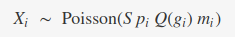
\includegraphics{images/poisson_sequencing_model.png}
	\caption{Вероятностая модель числа прочтений $X_i$ в сегменте $i$ в DNA-seq. $S$ — \textit{scale factor}, $p_i$ — число копий сегмента, $Q(g_i)$ — влияние \textit{GC-состав}, $m_i$ — \textit{bin mappability}}
\end{figure} 

Ниже приведены определения этих факторов:

\begin{definition}[\textit{Scale factor}]
	Число ридов, которые фрагмент ДНК порождает при секвенировании. Эта величина зависит как от \textbf{сложности библиотеки} (матожидание числа различных молекул, которые могут получиться в ходе ПЦР), так и от \textbf{глубины секвенирования} (точное значение зависит от технологии, но неформально стоит понимать как число ридов на единицу длины; увеличение амплификации повышает глубину покрытия, но и увеличивает затраты).
\end{definition}

\begin{definition}[\textit{Bin mappability}]
	Bin mappability неформально следует понимать как долю $k$-меров из заданного диапазона, которые однозначно выравниваются на этот же диапазон, где $k$ подчиняется Пуассоновской модели данных секвенирования. Если диапазон состоит из повторов одного короткого участка, то его mappability будет низкой, так как однозначно выравниваться будут только риды длиной больше половины от размера этого диапазона, вероятность которых будет мала. При заданной сегментации, эту величину можно с заданной точностью посчитать аналитически, но обычно для этого используют метод Монте-Карло.
\end{definition}

\begin{definition}[\textit{GC-состав}]
	Доля гуанина (G) и цитозина (C) среди нуклеотидов последовательности. В комплементарной GC-паре три водородных связи вместо двух как у AT-пар, потому последовательности с высоким содержанием G и C более устойчивы к нагреву, а потому реже расщепляются на фрагменты, достаточно короткие для амплификации при ПЦР. Аналогично, если GC-состав очень мал, то велик шанс, что при нагреве последовательность распадётся на слишком маленькие части, к которым уже нельзя будет присоединить праймер. Как следствие, покрытие последовательностей со слишком большим или слишком маленьким GC-составом в среднем ниже.
	\begin{figure}[H]
		\centering
		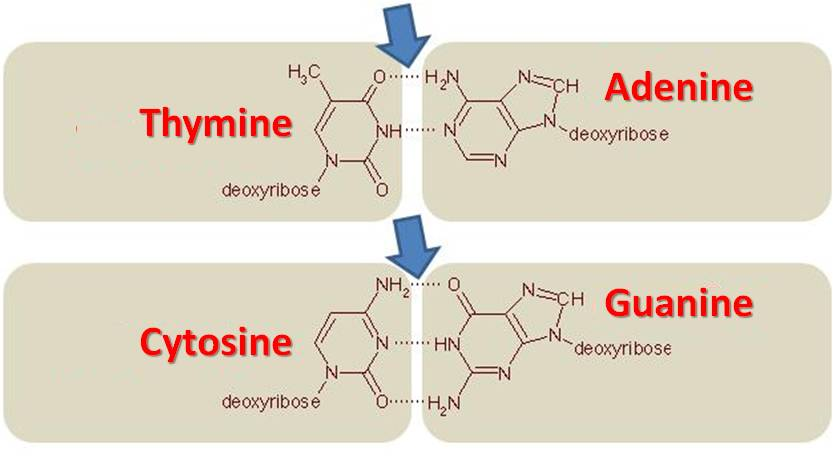
\includegraphics[keepaspectratio=true,scale=0.5]{images/gc_content.jpg}
		\caption{Комлементарные пары: аденин-тимин и гуанин-цитозин}
	\end{figure}
\end{definition}

В случае RNA-seq простой модели, к сожалению, быть не может. Дело в том, что геном статичен. Факторов, которые могут повлиять на распределение ридов в DNA-seq, не так много: это либо структурные вариации, либо особенности нуклеотидной последовательности как строки, без привязки к её биологическому смыслу. Картина экспрессии же постоянно меняется. На неё влияет и клеточный цикл, и окружающая среда, и патологии отдельных компонент клетки. Многочисленные регуляторные механизмы не позволяют моделировать экспрессию генов по отдельности: уровни экспрессии часто коррелируют, а иногда и зависят друг от друга нелинейно (т.н. \textbf{синергия генов}). Хуже того, в науке хорошо изучено такое явление как \textbf{эпистаз} — мутации в одном гене могут приводить к качественным изменениям фенотипа, выходящим далеко за пределы непосредственных функций этого гена. В современной науке существует множество моделей транскрипции, принимающих во внимание многие из этих факторов, но их содержательный обзор выходит далеко за рамки данной работы. 

\subsection{Алгоритмы предобработки данных}
Профессия вычислительного биолога подразумевает рутинную обработку больших гетерогенных данных, особенно что касается single-cell технологий. В связи с этим был реализован протокол предобработки данных секвенирования, основные шаги которого разобраны в данном разделе.
\begin{figure}[H]
	\centering
	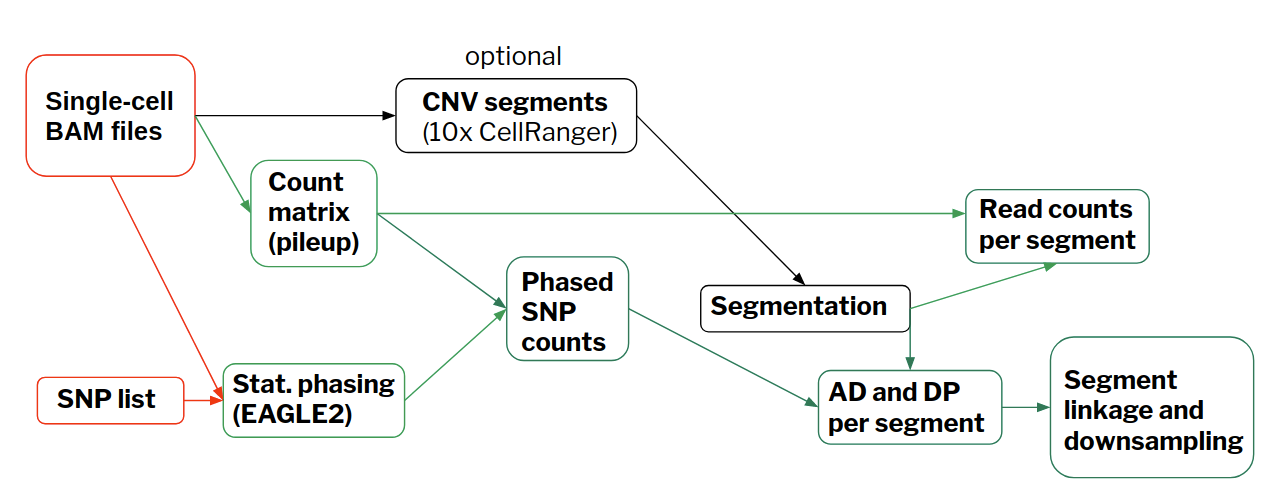
\includegraphics[keepaspectratio=true,scale=0.4]{images/preprocessing_pipeline.png}
	\caption{Граф протокола предобработки данных для алгоритма XClone. Красным обозначены входные данные, чёрным — опциональные шаги, зелёным — реализованные стадии.}
\end{figure}
\subsubsection{Извлечение данных из BAM-файлов}
\textbf{BAM} — \textit{binary SAM — binary sequence alignment/map format} — общепринятый формат сжатого хранения данных секвенирования, c подробностями которого можно ознакомиться в оригинальной публикации \cite{Samtools}. BAM-файл, полученный по протоколам 10x Genomics, занимает до нескольких терабайтов дискового пространства, потому эффективное извлечение информации из BAM-файлов это нетривиальная инженерная задача. Главные входные файлы XClone — матрицы прочтений. Таких матриц требуется три:
\begin{itemize}
	\item матрица $\mathrm{RD}$ всех прочтений достаточного качества;
	\item матрица $\mathrm{DP}$ всех прочтений, накрывающих хоть один ОНП в пределах сегментов; 
	\item матрица $\mathrm{AD}$ всех прочтений, накрывающих хоть альтернативный аллель ОНП в пределах сегментов.
\end{itemize}
Для получения матрицы $\mathrm{RD}$ из данных scRNA-seq был использован протокол \textbf{count} из \textbf{CellRanger}. Для всех остальных матриц во всех остальных случаях был использован \textbf{CellSNP}\footnote{https://github.com/single-cell-genetics/cellSNP}. 
\subsubsection{Статистическое фазирование гаплотипов} 
Гаплотипирование — определение того, от какого родителя унаследован каждый алллель в геноме — одна из ключевых задач генетики человека. Сложность её решения обусловлена контекстом, в котором она возникает в современных исследованиях, когда секвенируются порядка $2\cdot 10^{4}$ — $10^{6}$ позиций в геномах тысяч человек. Если прочтения короткие и не накрывают много позиций одновременно, то нужно секвенировать обоих родителей каждого участника эксперимента, что непрактично и не всегда возможно. Следовательно, нужно разрабатывать статистические методы гаплотипирования. Они основаны на наблюдении, что некоторые группы аллелей часто наследуются совместно. Это явление называется \textbf{неравновесной сцепленностью}. Если прогаплотипировано достаточное количество представителей популяции, то можно построить приближённые таблицы сцепленности и гаплотипировать новые образцы методом максимизации правдоподобия. 

На момент написания этого текста, стандартом статистического гаплотипирования считается алгоритм \textbf{EAGLE2}\cite{Eagle2}\footnote{https://data.broadinstitute.org/alkesgroup/Eagle/}. Этот алгоритм основан на скрытых марковских моделях и использует 32,470 образца из базы данных \textbf{Haplotype Reference Consortium}\cite{HaplotypeReferenceConsortium}.

Алгоритм EAGLE2 обладает существенным недостатком: его метки имеют только локальный смысл. В пределах окна в 20-50 килобаз любые два ОНП с одинаковой наследуются совместно, но при сдвиге окна смысл меток может спонтанно поменяться на противоположный, это так называемая \textbf{ошибка смены цепи}. Т.е. два ОНП с разных концов хромосомы, помеченые одной меткой, могут быть унаследованы от разных родителей. Из-за этого в матрицах прочтений размывается сигнал аллельного дисбаланса: чтобы сделать данные менее разреженными, прочтения соседних небольших сегментов суммируются, в том числе и аллель-специфичные. Ясно, что если среди двух соседних сегментов с одинаковой меткой один полностью унаследован от отца, а второй — от матери, то при сложении их аллель-специфичные сигналы скомпенсируют друг друга. Это, в свою очередь, приводит к неправильному предсказанию аллель-специфичных структурных вариаций и неправильной кластеризации клеток. Авторы EAGLE2 в переписке явно дали понять, что в общем случае  детектировать и исправлять такого рода ошибки их подход не позволяет. Но в контексте модели XClone удалось разработать статистический метод, показавший хорошие результаты при устранении ошибок смены цепи. Его подробное описание можно найти в одноимённом разделе.

\subsubsection{Подходы к сегментации генома}
Одной из основных задач XClone является предсказание \textbf{ASCNV} — аллель-специфических структурных вариаций генома. Это происходит в несколько этапов: (1) вначале производится сегментация генома с одновременным подсчётом матриц прочтений, (2) затем глубина покрытия сегментов сравнивается с эталонной для подсчёта RDR, (3) откуда получается оценка общего числа копий, (4) которая затем уточняется при помощи сигналов аллельного дисбаланса. Тем не менее, на точность предсказания влияют ещё и технические факторы, фигурирующие в вероятностной модели числа прочтений. Наиболее существенным фактором является bin mappability.

Подсчёт bin mappability — задача чисто техническая и довольно утомительная, т.к. она подразумевает проведение симуляций процесса секвенирования по какому-то конкретному протоколу. Кроме того, она давно считается решённой, а потому не представляет особого научного интереса. В связи с этим, для отфильтровывания участков низкого качества используется готовое решение — \textbf{CellRanger DNA}, алгоритм\footnote{https://support.10xgenomics.com/single-cell-dna/software/pipelines/\\latest/algorithms/cnv\_calling} от 10X Genomics, поставщика оборудования для single-cell севенирования в научной группе автора. Этот алгоритм разбивает геном на сегменты длиной в 20кб, после чего отфильтровывает те, для которых bin mappability меньше, чем 70\% (не более 10-15\% при использовании референсного генома GRCh37). CellRanger DNA сам по себе является алгоритмом поиска CNV. Тем не менее, он размечает максимально возможную часть генома каждой из клеток, в том числе участки без структурных вариантов. Благодаря этому можно гарантировать, что все участки генома, пригодные для надёжного определения ASCNV, войдут в итоговую сегментацию. 

Найденные участки накрывают некоторое подмножество референсного генома, которое затем подразделяется на сегменты размера 20-50 килобаз, в пределах которых вероятность ошибки смены цепи невелика, а потому сигнал аллельного дисбаланса статистически достоверный.

\begin{figure}[H]
	\centering
	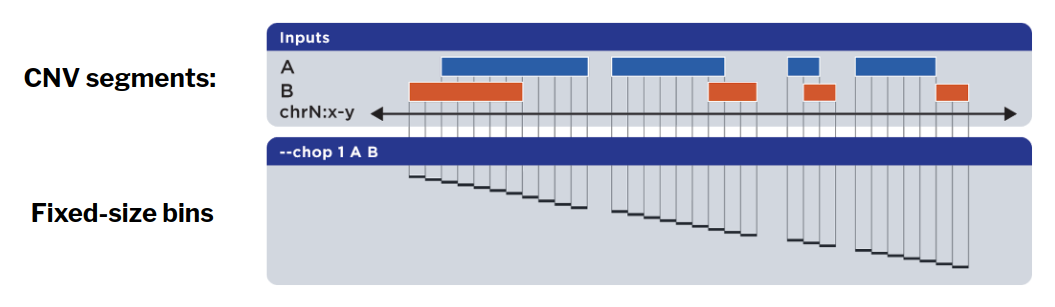
\includegraphics[keepaspectratio=true,scale=0.4]{images/segmentation.png}
	\caption{Иллюстрация алгоритма сегментирования генома. Длина индивидуальных сегментов задаётся заранее и выбирается из диапазона 20-50кб. Каждые $ k $ подряд идущих фрагментов затем объединяются в блоки. Соответствующие подматрицы прочтений при этом суммируются с одновременной коррекцией ошибок смены цепи.}
\end{figure}

В силу того, что структурные вариации обычно охватывают участки генома размеров хотя бы в несколько мегабаз, перед началом предсказания уместно аггрегировать подряд идущие сегменты в блоки фиксированного размера (обычно 1-5 мегабаз), чтобы получить менее шумные BAF и RDR. Тем не менее, наивно аггрегировать содержимое сегментов внутри блока — просуммировать числа прочтений — не получится, т.к. можно потерять аллель-специфический сигнал из-за ошибок смены цепи. В связи с этим был разработан алгоритм суммирования с коррекцией ошибок, который разобран в следующем разделе.

Такой подход к сегментации генома используется в заключительной версии XClone. Тем не менее, изначально большие надежды возлагались на более продвинутый метод, основанный на данных секвенирования длинными прочтениями по технологии Oxford Nanopore. Если прочтения достаточно длинные, они могут накрывать сразу несколько ОНП. Благодаря этому их гаплотипы определяются однозначно: просто из нуклеиотидной последовательности рида понятно, какие именно аллели лежат на одной хромосоме. Если покрытие генома достаточно хорошее, то длинные прочтения будут накладываться друг на друга, за счёт чего можно получить достаточно длинные гаплотипы. В силу того, что в первой версии модели ASCNV считались известными, как и клональные линии клеток в DNA-seq образце, для получения итоговой сегментации диапазоны структурных вариаций, обнаруженных CellRanger DNA, пересекались с гаплотипами, полученными по данным Oxford Nanopore. 

\begin{figure}[H]
	\centering
	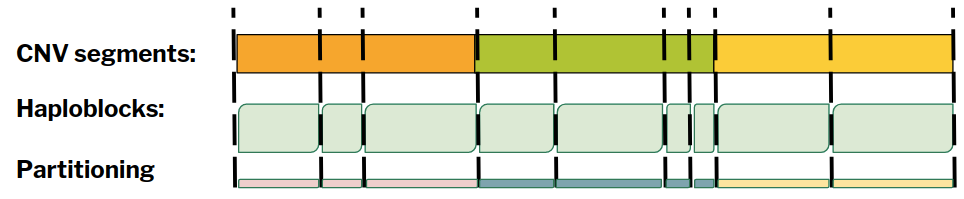
\includegraphics[keepaspectratio=true,scale=0.4]{images/cnv_haploblock_segmentation.png}
	\caption{Сегментирование генома в первоначальной версии XClone. Гаплотипические блоки, найденные по данным Oxford Nanopore DNA-seq, пересекаются с диапазонами структурных вариаций, найденных CellRanger DNA.}
\end{figure}

Тем не менее, такой подход оказался хорош лишь в теории. На практике, найденные таким способом гаплотипические блоки оказывались слишком короткими, порядка нескольких килобаз. Кроме того, распределение их длин имело достаточно большую дисперсию, что доставляло неудобства как при реализации, так и при интерпретации результатов: чем меньше сегмент, тем более зашумленный от него исходит сигнал. Когда таких сегментов много, модель переобучалась на шум в них, что приводило к неадекватному предсказанию меток классов. 

\subsubsection{Исправление ошибок смены цепи}\label{bin_linkage_em}
Поскольку одной из главных задач XClone является предсказание \textit{аллель-специфичных} структурных вариаций в геноме, матрицы $\mathrm{AD}$ и $\mathrm{DP}$ аллель-специфичных прочтений должны отражать биологию аллельного дисбаланса в клетках образца. Для этого нужно понимать, к какому гаплотипу принадлежит каждый ОНП. В разделе про статистическое гаплотипирование ОНП был сделан акцент на том, что существующие алгоритмы гарантируют только локальную корректность: при использовании алгоритма EAGLE2, следует ожидать, что при разбиении хромосомы на непересекающиеся окна длины 20-50 килобаз все гетерозиготные ОНП в пределах одного окна будут иметь одинаковый гаплотип, если это на самом деле так. Тем не менее, гаплотипы соседних сегментов с точки зрения алгоритма могут не совпадать даже тогда, когда на самом деле должны. К этому приводят так называемые \textbf{ошибки смены цепи} (\textit{switching error}) — спонтанная и неявная замена гаплотипических меток на противоположные внутри алгоритма. Классификацию ошибок смены цепи можно найти в статье \cite{Choi2018Plos}, цитата из которой приведена ниже:

\textit{"Phasing accuracy is typically measured by counting the number of \textbf{‘switches’} between known maternal and paternal haplotypes that should not occur if individual maternal and paternal chromosomal nucleotide sequence content has been accurately characterized. If an inconsistency is identified, then it is called a ‘switch error.’ These switch errors manifest themselves as induced and false recombination events in the inferred haplotypes compared with the true haplotypes. To identify \textbf{switch errors}, the phase of each site is compared with upstream neighboring phased sites. The switch error rate (SER) is defined as the number of switch errors divided by the number of opportunities for switch errors. Switch errors were further classified into three categories: \textbf{long}, \textbf{point}, and \textbf{undetermined}. A long switch appears as a large-scale pseudo recombination event; that is, there are no other switches in the local neighborhood around the long switch (e.g., no other switches within three consecutive heterozygous sites). On the contrary, a small-scale switch error appearing as two neighboring switch errors is considered as a point switch (e.g., two switches within three consecutive heterozygous sites, with the pair of switches counted as a point switch). The remaining switches are considered undetermined (e.g., only two sites phased in a small phasing block, so the switch error could not be classified into long or point)."}

Тем не менее, разбиение генома на фрагменты по 20-50 килобаз непрактично: в силу разреженности данных, это даёт  слабый и зашумленный сигнал аллельного дисбаланса. В связи с этим был разработан метод, одновременно решающий обе описанные проблем. На первом шаге алгоритма происходит разбиение генома на непересекающиеся сплошные сегменты длины $L$. Затем каждые $N$ подряд идущих сегментов объединяются в блок длины $NL$. В пределах блока переключения моделируются бернуллиевскими случайными величинами, по одной на каждый сегмент. Параметры этих распределений, в свою очередь, выводятся \textbf{ЕМ-алгоритмом}. После исправления ошибок, прочтения сегментов внутри блока суммируются, что даёт более стабильный сигнал. Эта идея была сформулирована в \cite{ChiselBiorxiv}, но технические детали были осознанно исключены авторами CHISEL из препринта. 

Прежде чем приступать к рассмотрению метода, сформулируем необходимые определения:

\begin{definition}[\textit{ЕМ-алгоритм}]$  $\\
EM-алгоритм (от английского \textit{"EM"} — \textit{"Expectation Maximization"}) — метод поиска оценок максимального правдоподобия (ОМП) или оценок апостериорного максимума (ОАП) параметров статистических моделей, содержащих скрытые переменные. 

\begin{algorithm}[H]
	\SetAlgoLined
	\KwResult{$\bm{\Theta}^{\ast},\ p(\bm{Z}\ |\ \bm{X}, \bm{\Theta}^{\ast})$}
	\text{$t = 0$}\;
	\text{$\bm{\Theta}^{(0)}$ инициализируется случайно}\;
	\While{$Q(\bm{\Theta}^{(t+1)}\ |\ \bm{\Theta}^{(t+1)}) - Q(\bm{\Theta}^{(t)}\ |\ \bm{\Theta}^{(t)}) > \eps$}{
		$\mathcal{L}(\bm{\Theta}^{(t)}; \bm{Z}, \bm{X}) := p(\bm{X}, \bm{Z}\ |\ \bm{\Theta}^{(t)})$\;
		$Q(\bm{\Theta}\ |\ \bm{\Theta}^{(t)}) := \mathbb{E}_{\bm{Z} | \bm{X}, \bm{\Theta}^{(t)}} \log \mathcal{L}(\bm{\Theta}; \bm{Z}, \bm{X})$ \tcp{E-шаг}
		$\bm{\Theta}^{(t+1)} := \arg\max\limits_{\bm{\Theta}} Q(\bm{\Theta}\ |\ \bm{\Theta}^{(t)})$ \tcp{M-шаг}
		$t = t + 1$
	}
	$\bm{\Theta}^{\ast} := \bm{\Theta}^{(t)}$
	\caption{ЕМ-алгоритм в общем виде}
\end{algorithm}

Здесь $\bm{Z}$ — дискретные скрытые переменные, $\bm{\Theta}$ — параметры статистической модели, $\bm{X}$ — выборка, $\eps > 0$, $p$ — функция плотности. Каждая итерация алгоритма состоит из двух основных шагов:
\begin{enumerate}
	\item \textbf{Е-шаг}, на котором устраняется явная зависимость от скрытых переменных посредством взятия матожидания логарифма совместной функции правдоподобия по условному распределению $\bm{Z}\ |\ \bm{X}, \bm{\Theta}^{(t)}$;
	\item \textbf{M-шаг}, на котором параметры нового апостериорного распределения $\bm{\Theta}^{(t+1)}$ выбираются таким образом, чтобы максимизировать $ Q(\bm{\Theta}, \bm{\Theta}^{(t)}) $ — функцию правдоподобия "в среднем". 
\end{enumerate}
\end{definition}

С теоретическим обоснованием и формальным доказательством корректности EM-алгоритма можно ознакомиться в (\cite{MurphyProbabilisticML}, стр. 363-365). В контексте решаемой задачи $\bm{X}, \bm{Z}, \bm{\Theta}$ имеют следующий смысл:
\begin{itemize}
	\item $\bm{Z} = \{z_{1}, \ldots, z_{N}\}$ — независимые в совокупности индикаторы корректности гаплотипов сегментов
	\begin{gather*}
			\forall i: z_i \sim \mathrm{Bern}(p_i)\\
			\forall q \in \{0, 1\}^{N}: p(\bm{Z} = q\ |\ p_1, \ldots, p_n) = \prod_{i=1}^{N} p(z_i = q_i\ |\ p_i) = \prod_{i=1}^{N} p_i^{q_i} ( 1 - p_i)^{1-q_i}
	\end{gather*}
	Если $z_i = 1$, то будем говорить, что сегмент $i$ имеет корректный гаплотип, иначе — инвертированный. Эти обозначения имеют смысл только в пределах одного блока, в соседних блоках метки могут иметь противоположный смысл. Из этого наблюдения становится ясно, что алгоритм не решает проблему переключения полностью, но уменьшает число ошибок за счёт аггрегации сегментов в блоки.
	\item Обозначим через $M$ число клеток образца, тогда $\bm{X} = (\bm{X}_{1}, \ldots, \bm{X}_{M}),\ X_{c} := (\bm{a}_c, \bm{b}_c)$ —  вектора прочтений для каждой из клеток, по компоненте на сегмент.  $\bm{a}_c = (a_{c, 1}, \ldots, a_{c, N})$ — число прочтений аллеля А (альтернативный аллель), $\bm{b}_c =  (b_{c, 1}, \ldots, b_{c, N})$ — аллеля Б (референсный аллель).
	\item $\forall c \in \overline{1, M}: \bm{r}_c := \bm{a}_{c} + \bm{b}_{c}$ — вектора прочтений обоих аллелей вместе.
	\item $\bm{\Theta} = (\theta_1, \ldots, \theta_M; p_1, \ldots, p_N)$, где $\theta_c$ — пропорция ридов гаплотипа 1 в блоке в клетке $c$. Алгоритм предполагает, что пропорция гаплотипа 1 одинакова во всех сегментах внутри блока с точностью до переключения.
\end{itemize}
	
В этих обозначениях можно сформулировать и доказать следующее утверждение:
\begin{claim}
	Правила пересчёта параметров апостериорного распределения на М-шаге ЕМ-алгоритма имеют вид:
	\begin{equation}
		\begin{aligned}
			p_{i}^{(t+1)} &= \dfrac{ p_{i}^{(t)} \prod_{c=1}^{M} (\theta_{c}^{(t)})^{a_{c, i}} (1 - \theta_{c}^{(t)})^{b_{c, i}}}{p_{i}^{(t)} \prod_{c=1}^{M} (\theta_{c}^{(t)})^{a_{c, i}} (1 - \theta_{c}^{(t)})^{b_{c, i}} + (1 - p_{i}^{(t)}) \prod_{c=1}^{M} (\theta_{c}^{(t)})^{b_{c, i}} (1 - \theta_{c}^{(t)})^{a_{c, i}}}\\
			\theta_c^{(t+1)} &= \frac{\sum_{i=1}^{N}a_{i,c} \gamma^{(t)}_{i,1} + b_{i,c} \gamma^{(t)}_{i,0}}{\sum_{i=1}^{N} r_{i,c}}
		\end{aligned}
		\label{em_update_rules}
	\end{equation}
	где $\forall j \in \{0, 1\}: \gamma^{(t)}_{i,j} := P(z_i = j\ |\ \bm{X}, \bm{\Theta}^{(t)})$.
\end{claim}
\begin{proof}
  Вектора прочтений в клетках независимы в совокупности, потому: 
	\begin{gather*}
			P(\bm{X}\ |\ \bm{Z}, \bm{\Theta}) = \prod_{c=1}^{M} p(\bm{X}_c\ |\ \bm{Z}, \bm{\Theta}) = \prod_{c=1}^{N} \theta_{c}^{\widehat{a}_c(\bm{Z})}(1 - \theta_{c})^{\widehat{b}_c(\bm{Z})}
	\end{gather*}
	Где 
	\begin{gather*}
	\begin{cases}
		\widehat{a}_c(\bm{Z}) := \sum_{i=1}^{N} \left[z_i a_{c, i} + (1 - z_i) b_{c, i} \right],\\
		\widehat{b}_c(\bm{Z}) := \sum_{i=1}^{N} \left[(1 - z_i) a_{c, i} + z_i b_{c, i} \right],\\
		c \in \overline{1, M}
	\end{cases}
	\end{gather*}
	Тогда функция правдоподобия и её логарифм принимают вид
	\begin{align*}
			&\mathcal{L}(\bm{\Theta}; \bm{X}, \bm{Z}) = p(\bm{X}, \bm{Z} \ |\ \bm{\Theta}) = p(\bm{X}\ |\ \bm{Z}, \bm{\Theta}) p(\bm{Z}\ |\ \bm{\Theta})\\
			&l(\bm{\Theta}; \bm{X}, \bm{Z}) = \log \mathcal{L}(\bm{\Theta}; \bm{X}, \bm{Z}) =\\
			&= \log \prod_{\bm{q} \in \{0, 1\}^{N}} \left(\prod_{c=1}^{M} \theta_{c}^{\widehat{a}_c(\bm{q})}(1-\theta_{c})^{\widehat{b}_c(\bm{q})} \prod_{i=1}^{N} p_i^{q_i}(1-p_i)^{1-q_i}\right)^{\mathbb{I}\{\bm{Z} = \bm{q}\}} =\\
			&=\sum_{\bm{q} \in \{0, 1\}^{N}} \mathbb{I}\{\bm{Z} = \bm{q}\} \left( \sum_{c=1}^{M}\sum_{i=1}^{N} \widehat{a}_{c,i}(\bm{q}) \log \theta_{c} + \widehat{b}_{c,i}(\bm{q}) \log (1-\theta_{c})\right) +\\
			&+ \sum_{\bm{q} \in \{0, 1\}^{N}} \mathbb{I}\{\bm{Z} = \bm{q}\} \left(\sum_{i=1}^{N} q_{i} \log p_{i} + (1 - q_{i}) \log (1 - p_{i}) \right)
	\end{align*}
	Изменением порядка суммирования можно показать, что каждая из этих двух сумм распадается на $N$ сумм поменьше, по одной на каждую из скрытых переменных. В следствие этого и того, что компоненты случайного вектора $ \bm{Z} $ независимы в совокупности, шаги EM-алгоритма имеют вид:\\
	\noindent \textbf{E-шаг:}
	\begin{align*}
		&p(\bm{Z}\ |\ \bm{X}, \bm{\Theta}^{(t)})\ \propto\ p(\bm{X}\ |\ \bm{Z}, \bm{\Theta}^{(t)}) p(\bm{Z}\ |\ \bm{\Theta}^{(t)}) \implies\\
		&\implies \E_{\bm{Z}|\bm{X}, \bm{\Theta}^{(t)}} l(\bm{\Theta}; \bm{Z}, \bm{X}) = \sum_{i=1}^{N} \E_{\bm{z}_i|\bm{X}_i, \bm{\Theta}^{(t)}} \log \mathcal{L}(\bm{\Theta}; \bm{z}_i, \bm{X}_i) =\\
		&= \sum_{i=1}^{N} \sum_{q_i = 0}^{1} p(\bm{z}_i = q_i\ |\ \bm{X}_i, \bm{\Theta}^{(t)}) \left(
		\begin{aligned}
			&\sum_{c=1}^{M} \left[ \widehat{a}_{c,i}(q_i) \log \theta_{c} + \widehat{b}_{c,i}(q_i) \log (1 - \theta_{c}) \right] +\\
			&+ \log p(\bm{z}_i = q_i\ |\ \bm{\Theta})
		\end{aligned} \right) =\\
		&= \sum_{i=1}^{N} \left[ 
		\begin{aligned}
			&\gamma_{i,1}^{(t)} \left( \sum_{c=1}^{M} \left[a_{c,i} \log \theta_c + b_{c,i} \log(1-\theta_c) \right] + \log p_i \right) +\\ 
			&+ \gamma_{i,0}^{(t)} \left( \sum_{c=1}^{M} \left[b_{c,i} \log \theta_c + a_{c,i} \log(1-\theta_c) \right] + \log (1 - p_i) \right) 
		\end{aligned}
		\right] = Q(\bm{\Theta}\ |\ \bm{\Theta}^{(t)})
	\end{align*}
	
	\noindent \textbf{M-шаг:}
	\begin{gather*}
		p_{i}^{(t+1)} = \arg\max_{p_{i}} Q(\bm{\Theta}\ |\ \bm{\Theta}^{(t)}) \iff \frac{\gamma_{i, 1}^{(t)}}{p_{i}^{(t+1)}} - \frac{\gamma_{i, 0}^{(t)}}{1 - p_{i}^{(t+1)}} = 0 \iff p_{i}^{(t+1)} = \gamma_{i, 1}^{(t)}\\
		\begin{aligned}
			\theta_{c}^{(t+1)} = \arg\max_{\theta_c} Q(\bm{\Theta}\ |\ \bm{\Theta}^{(t)}) &\iff \frac{\sum_{i=1}^{N} \gamma_{i,1}^{(t)} a_{c, i} + \gamma_{i,0}^{(t)} b_{c, i}}{\theta_{c}^{(t+1)}} - \frac{\sum_{i=1}^{N} \gamma_{i,1}^{(t)} b_{c, i} + \gamma_{i,0}^{(t)} a_{c, i}}{1 - \theta_{c}^{(t+1)}} = 0\\
			&\iff \theta_c^{(t+1)} = \frac{\sum_{i=1}^{N} \gamma_{i,1}^{(t)} a_{c, i} + \gamma_{i,0}^{(t)} b_{c, i}}{\sum_{i=1}^{N} a_{c, i} +  b_{c, i}}
		\end{aligned}
	\end{gather*}
	Где необходимое условие локального экстремума является также достаточным в силу выпуклости функции $Q(\bm{\Theta}\ |\ \bm{\Theta}^{(t)})$ (\cite{MurphyProbabilisticML}, стр. 363-364).
\end{proof}

\begin{figure}[H]
	\centering
	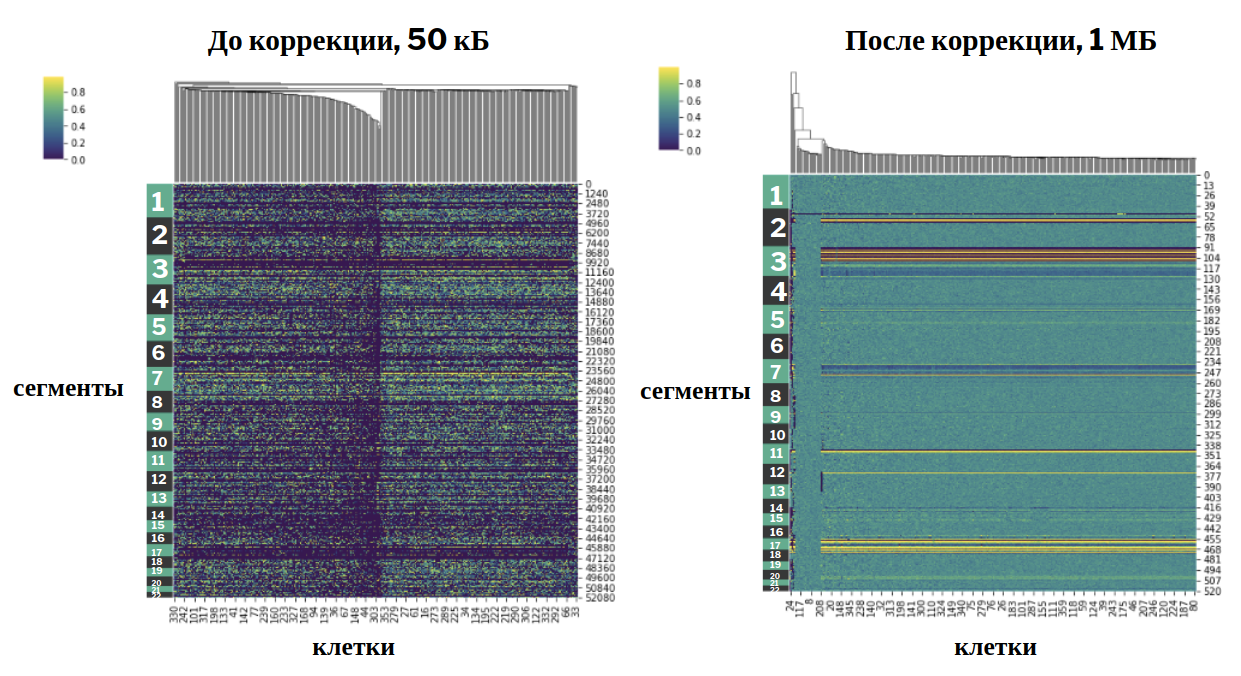
\includegraphics[keepaspectratio=true,scale=0.4]{images/bin_linkage.png}
	\caption{Коррекция ошибок смены цепи на примере ДНК-образца STP-Nuclei. На рисунке изображены тепловые карты долей аллеля из <<материнского>> гаплотипа, числа слева обозначают номер хромосомы. Картина аллельного дисбаланса до коррекции практически не прослеживается, после — становится очевидна.}
\end{figure}

После того, как значения $z_1, \ldots, z_N$ были определены по данным DNA-seq, их же можно использовать для предобработки данных RNA-seq, полученных из образцов тканей того же пациента. Это даёт возможность интеграции двух модальностей в единую статистическую модель.

Стоит отметить, что на практике $p_{i}^{(t+1)}$ следует считать по эквивалетной, но уже численно устойчивой формуле:
\begin{gather*}
	p_{i}^{(t+1)} = \left(1 + \exp\left[\log(1 - p_{i}^{(t)}) - \log(p_{i}^{(t)}) + \sum_{c=1}^{M} \Delta_{c, i} (\log(\theta_{c}^{(t)}) - \log(1 - \theta_{c}^{(t)}))\right]\right)^{-1}
\end{gather*}
Где $\Delta_{c, i} := b_{c, i} - a_{c, i}$, а показатель экспоненты стоит искусственно приводить к диапазону $[-C; C]$ для некоторого $C > 0$ (авторами было выбрано $C = 100$). В противном случае $\prod_{c=1}^{M} (\theta_{c}^{(t)})^{a_{c, i}} (1 - \theta_{c}^{(t)})^{b_{c, i}}$ может представлять собой произведение тысяч или даже миллионов очень маленьких величин в больших степенях. Стандартной реализации чисел с плавающей запятой двойной точности недостаточно для хранения результатов промежуточных вычислений при использовании наивной формулы. 
\subsection{Использованные данные}
\subsection{Первоначальная версия XClone: только ASE-модуль}

\subsubsection{Plate notation}
\subsubsection{Семплирование по Гиббсу}
\subsubsection{Предложенная модель, её недостатки}
\textbf{scDNA + CNV and scRNA, different samples}

\begin{figure}[h!]
	\centering
	\tikz{ %
		\node[obs] (nu) {${\nu_{l}}$}; %
		\node[latent, below=of nu] (Theta) {${\theta_{il}}$}; %
		\node[latent, fill=blue!20, left =of nu, xshift=-0.5cm] (I_G) {${I_{j}^G}$}; %
		\node[latent, right=of nu, xshift=0.5cm] (I_E) {${I_{h}^E}$}; %
		
		\node[latent, rectangle, below=of I_G] (P_G) {${p_{ij}^G}$} ; %
		\node[latent, rectangle, below=of I_E] (P_E) {${p_{ih}^E}$} ; %
		
		\node[latent, fill=blue!20, below=of Theta] (T) {${t_{ik}}$} ; %
		\node[obs, below=of P_G] (A_G) {${a_{ij}^G}$} ; %
		\node[obs, below=of P_E] (A_E) {${a_{ih}^E}$} ; %
		\node[obs, left=of A_G] (D_G) {${d_{ij}^G}$} ; %
		\node[obs, right=of A_E] (D_E) {${d_{ih}^E}$} ; %
		
		\edge {nu} {Theta} ; %
		\edge {I_G} {P_G} ; %
		\edge {I_E} {P_E} ; %
		\edge {Theta} {P_G} ; %
		\edge {T} {P_G} ; %
		\edge {Theta} {P_E} ; %
		\edge {T} {P_E} ; %
		\edge {P_G} {A_G} ; %
		\edge {D_G} {A_G} ; %
		\edge {P_E} {A_E} ; %
		\edge {D_E} {A_E} ; %
		
		
		{\tikzset{plate caption/.append style={below=5pt of #1.south east}};
			\plate[inner xsep=0.8cm, inner ysep=0.4cm, xshift=-0.6cm, yshift=0cm] {plate1} {(D_G) (A_G)(P_G)(D_E) (A_E)(P_E)} {CNV-haplo block $i$} };
		
		{\tikzset{plate caption/.append style={below=30pt of #1.south}};
			\plate[inner xsep=0.4cm, inner ysep=0.4cm, xshift=0.1cm, yshift=0.28cm, color=black] {plate1} {(D_G) (A_G)(P_G)(I_G)} {cell $j$ in scDNA} };
		{\tikzset{plate caption/.append style={below=30pt of #1.south}};
			\plate[inner xsep=0.4cm, inner ysep=0.4cm,  xshift=-0.1cm, yshift=0.28cm, color=black] {plate2} {(D_E) (A_E)(P_E)(I_E)} {cell $h$  in scRNA} };
		
		{\tikzset{plate caption/.append style={above=2pt of #1.north}};
			\plate[inner sep=0.25cm, xshift=0cm, yshift=0.12cm] {plate3} {(nu) (Theta)} {CNV $l$} };
		
		{\tikzset{plate caption/.append style={below=30pt of #1.south}};
			\plate[inner xsep=0.25cm, inner ysep=0.4cm,  xshift=0cm, yshift=0.2cm] {plate4} {(T)} {clone $k$} };
		%			
	}
\end{figure}

\noindent In this model, clonal assignment $ \mathbf{I^{G}} $ of cells in scDNA sample is assumed fixed. For each clone $ k $, for each same-CNV block $ i $ the clonal CNV state $ \mathbf{T}_{i,k} $ is defined to be the most frequent CNV state in that position across all cells assigned to clone $ k $. Clonal assignment $ \mathbf{I^{E}} $ in scRNA sample is learned.\\

\noindent This model learns the clonal structure in scRNA sample using ASE profiles from scDNA.

\textbf{Basic definitions}
\begin{enumerate}
	\item \textbf{Constants:}
	\begin{itemize}
		\item $ M^{G}, M^{E} $ — number of cells in scDNA and scRNA samples respectively.
		\item $ K $  — estimated number of clones in the sample.
		\item $ N $ — number of same-CNV blocks in scDNA sample (also used in scRNA sample).
		\item $ T_{\max} $ — maximal possible CNV number. User-defined with the default of 5.
		\item $ \tau $ — set of possible CNV configurations: 
		$$\{(1, 0), (0, 1), (2, 0), (1, 1), (1, 2), \ldots, T_{\max}, 0), \ldots, (0, T_{\max}) \}$$ The case of zero CNV number should be treated with care if we can't say for sure whether the part of the chromosome (both arms) is deleted).
	\end{itemize}
	\item \textbf{Other known quantities:}
	\begin{itemize}
		\item $ \mathbf{D^{G}}, \mathbf{D^{E}} $ — total read counts. To get a count of the block, one simply adds up the counts of the variants within the block. Here we assume that variants are far enough from each other, so that almost no reads overlap two variants at the same time. Otherwise, adding things up wouldn't make sense.
		\item $ \mathbf{A^{G}},\ \mathbf{A^{E}} $ — same for allele-specific counts.
		\item $ \textbf{f} = (f_1, \ldots, f_K)$ — $K$-dimensional vector of estimated clonal fractions ($ \sum_{i=1}^{K} f_i = 1 $) 
		\item $ \mathbf{T} $ — CNV states of blocks ($\mathbf{T_{i,k}}$ is a CNV state of a block $ i $ in clone $ k $).
	\end{itemize}
	\item \textbf{Inferred quantities:}
	\begin{itemize}
		\item $ \mathbf{\Theta} $ — allelic rates of variants located within blocks of fixed CNV status. $ \mathbf{\Theta_{i,t}} $ is an allelic rate of a block $i$ with a CNV status $t$. Set of blocks for each clone is unique. Blocks are ordered as tuples of the form (\textit{block start, block length}).
		\item $ \mathbf{I^{E}} \in [K]^{M} $ — cell-to-clone assignment in scRNA sample.
	\end{itemize}
	\item \textbf{Some notational conventions:}
	\begin{itemize}
		\item Capitalized letter without superscript (like $ \mathbf{\Theta} $) denotes the information for both samples.
		\item $ \mathbf{H^{G}}, \mathbf{H^{E}} $ — CNV status of the blocks in accordance with the current label assignment: 
		$$ 
			\mathbf{H^{G}_{i,j}} := \mathbf{T_{i, I^{G}_{j}}},\quad \mathbf{H^{E}_{i,j}} := \mathbf{T_{i, I^{E}_{j}}}
		$$
		\item  $ \mathbf{X^{G}},\ \mathbf{X^{E}} $ — a shortcut to simplify the notation: $\mathbf{X^{G|E}_{i,j}}$ is an allelic rate of a block $ i $ in cell $ j $ based of the current cell-to-clone label assignment.
		$$ 
			\mathbf{X^{G}_{i,j}} := \mathbf{\Theta_{i, H^{G}_{i,j}}},\quad \mathbf{X^{E}_{i,j}} := \mathbf{\Theta_{i, H^{E}_{i,j}}} 
		$$
	\end{itemize}
\end{enumerate}
\textbf{Generative model formulation}
\begin{itemize}
	\item \textbf{Cell-to-clone assignment posterior:}
	\begin{equation}
		\P(\mathbf{I^{E}_{j}} = k_{0} \ |\  \mathbf{A_{j}}, \mathbf{D_{j}}, \mathbf{f}, \mathbf{\Theta}) =  
		\dfrac{\P(\mathbf{A_j} \ |\  \mathbf{D_j}, \mathbf{I^{E}_{j}} = k_{0}, \mathbf{\Theta}) \P(\mathbf{I^{E}_{j}} = k_{0} \ |\  \textbf{f}) }{\sum\limits_{k=1}^{K}\P(\mathbf{A_j} \ |\  \mathbf{D_j}, \mathbf{I^{E}_{j}} = k, \mathbf{\Theta}) \P(\mathbf{I^{E}_{j}} = k\ |\  \textbf{f}) }
	\end{equation}
	
	\item \textbf{ASE model:}
	\begin{equation}
		\begin{aligned}
			\P(\mathbf{A^{G}_{i,j}}\ |\ \mathbf{D^{G}_{i,j}}, \mathbf{\Theta}) &= \mathrm{Binom}(\mathbf{A^{G}_{i,j}}\ |\ \mathbf{D^{G}_{i,j}}, \mathbf{X^{G}_{i,j}})\\
			\P(\mathbf{A^{E}_{i,j}}\ |\ \mathbf{D^{E}_{i,j}}, \mathbf{\Theta}) &= \mathrm{Binom}(\mathbf{A^{E}_{i,j}}\ |\ \mathbf{D^{E}_{i,j}}, \mathbf{X^{E}_{i,j}}) 
		\end{aligned}
	\end{equation}
	
	\item \textbf{ASE likelihood (both terms factorize over variants):}
	\begin{equation}
		\begin{aligned}
			\P(\mathbf{A^{G}_{j}}\ |\ \mathbf{D^{G}_{j}}, \mathbf{I^{G}_{j}} = k^{G}, \mathbf{\Theta^{E}}) &= \prod_{i=1}^{N} \mathrm{Binom}(\mathbf{A^{G}_{j}}\ |\ \mathbf{D^{G}_{j}}, \mathbf{\Theta_{i, k^{G}}})\\
			\P(\mathbf{A^{E}_{j}}\ |\ \mathbf{D^{E}_{j}}, \mathbf{I^{E}_{j}} = k^{E}, \mathbf{\Theta}) &= \prod_{i=1}^{N} \mathrm{Binom}(\mathbf{A^{E}_{j}}\ |\ \mathbf{D^{E}_{j}}, \mathbf{\Theta_{i, k^{E}}})
		\end{aligned}
	\end{equation}
	
	\item \textbf{Allelic rate likelihood:} 
	\begin{equation}
		\begin{aligned}
			\mathcal{L}(\mathbf{\Theta}) &= \left (\prod_{j=1}^{M^{G}} \sum_{k^{G}=1}^{K}  \P(\mathbf{A^{G}_{j}}\ |\ \mathbf{D^{G}_{j}}, \mathbf{I^{G}_{j}} = k^{G}, \mathbf{\Theta}) \right ) \times\\
			&\times \left (\prod_{j=1}^{M^{E}} \sum_{k^{E}=1}^{K}  \P(\mathbf{A_{j}}\ |\ \mathbf{D^{E}_{j}}, \mathbf{I^{E}_{j}} = k^{E}, \mathbf{\Theta}) \cdot \P(\mathbf{I^{E}_{j}} = k^{E}\ |\ \mathbf{f}) \right ) 
		\end{aligned}
	\end{equation}
	To view the clonal assignment in a Bayesian way, we introduce informative prior $ \mathbf{\nu} $ for $\mathbf{\Theta}$.\\ 
	Using that <<posterior $ \propto $ prior $\times$ likelihood>>, we obtain:
	\begin{equation}
		\begin{aligned}
			&\P(\mathbf{\Theta}\ |\ \mathbf{A}, \mathbf{D}, \mathbf{f}, \mathbf{\nu}) \propto \P(\mathbf{\Theta}\ |\ \mathbf{\nu}) \times \mathcal{L}(\mathbf{\Theta}) =\\
			&= \prod_{l=1}^{N} \prod_{t\in\tau} \mathrm{Beta}(\alpha_{l,\tau}, \beta_{l,\tau}) \times \mathcal{L}(\mathbf{\Theta})
		\end{aligned}
	\end{equation}
	Parameters $\alpha_{t}, \beta_{t}$ are selected in such a way that the mode of $\mathrm{Beta}(\alpha_{t}, \beta_{t})$ equals to $ 1 / t $ \footnote{because if we assume that allelic rates only depend on the CNV status $ t $ then those rates could be computed as $ 1 / t $}.
\end{itemize}
\textbf{Selecting a prior for $\mathbf{\Theta}$}
CNV state of $t$ hides a plethora of possible configurations: it can mean "$ k $ copies of maternal chromosome and $ t - k $ copies of paternal" for any $ k \in \{0, \ldots, t\} $, all the variants are possible. But they are not equally possible: some are more supported by evidence than the rest. During initialization, for each block in each clone we should find the $ (k, t) $-configuration $ (k_0, t) $, such that $ k_0 / t $ is as close to the observed ASE ratio as possible. Then we choose values $ (\alpha, \beta) $ such that the mode of $ \mathrm{Beta}(\alpha, \beta) $, given by $ (\alpha - 1) / (\alpha + \beta - 2) $, equals to $ k_0 / t $. That means, we must solve the following problem:
$$
\dfrac{\alpha - 1}{\alpha + \beta - 2} = \frac{k_0}{t},\ \alpha \ge 1,\ \beta \ge 1
$$
Let's derive the solution. If $ k_0 = 0 $, it is clear that $ \alpha = 1 $, while any $ \beta > 1 $ works\footnote{Nevertheless, it is not clear which one to choose. As we try to reduce prior bias, let's set it to be equal $ 1 + \eps $  for some reasonable $ \eps > 0 $}. Otherwise:
\begin{equation}
\begin{aligned}
(\alpha - 1) t &= (\alpha + \beta - 2) k_0\\
k_0 \beta &= (t - k_0) \alpha -t + 2 k_0\\
\beta &= \left (\frac{t}{k_0} - 1\right ) \alpha - \left (\frac{t}{k_0} - 2 \right )\\
&\implies \alpha = 1 + \frac{t - 2k_0}{t - k_0},\ \beta = 1
\end{aligned}
\end{equation}
As $ \beta $ is linearly dependent from $ \alpha $, any increase in $ \alpha $ will pull $ \beta $ up, "sharpening" the shape of the distribution and making it more biased, thereby we decided to choose the minimal feasible $ \alpha $.\\
\textbf{Inference (Gibbs sampler)}
To use a Gibbs sampler, we define conditional probability distribution for each scalar random variable:\\
\textbf{Cell-to-clone label assignment:} 
\begin{equation}
	\begin{aligned}
		\P(\mathbf{I^{E}_j} = k\ |\ \mathbf{I^{E}_{-j}}, \mathbf{A^{E}}, \mathbf{D^{E}}, \mathbf{f}, \mathbf{\Theta}) 
		&\propto \P(\mathbf{A^{E}_{j}}\ |\ \mathbf{D^{E}_{j}}, \mathbf{I^{E}_{j}} = k, \mathbf{\Theta}) \cdot \P(\mathbf{I^{E}_{j}} = k\ |\ \mathbf{f}) 
	\end{aligned}
\end{equation}
\textbf{Allelic rates:}
Assuming fixed assignment, let's expand the joint likelihood equation: 
\begin{equation}
	\begin{aligned}
		&\P(\mathbf{\Theta}\ |\ \mathbf{A}, \mathbf{D}, \mathbf{I^{G}}, \mathbf{I^{E}}, \mathbf{f}, \mathbf{\nu}) \propto\\
		&\propto \left\{\prod_{l=1}^{N} \prod_{t\in \tau}\mathrm{Beta}(\alpha_{T_{l,t}}, \beta_{T_{l,t}}) \right\} 
		\left[ \prod_{j^{G}=1}^{M^{G}} \P(\mathbf{A^{G}_{j^{G}}}\ |\ \mathbf{D^{G}_{j^{G}}}, \mathbf{I^{G}_{j^{G}}}, \mathbf{\Theta}) \right] 
		\left[\prod_{j^{E}=1}^{M^{E}} \P(\mathbf{A^{E}_{j^{E}}}\ |\ \mathbf{D^{E}_{j^{E}}}, \mathbf{I^{E}_{j^{E}}}, \mathbf{\Theta}) \right]  =\\
		&= \prod_{l=1}^{N} \prod_{t\in \tau} \mathrm{Beta}(\alpha_{T_{l,t}}, \beta_{T_{l,t}}) 
		\left[ \prod_{j^{G}=1}^{M^{G}} \mathrm{Binom}(\mathbf{A^{G}_{j^{G}}}\ |\ \mathbf{D^{G}_{j^{G}}}, \mathbf{\Theta_{i, t}}) \right] \left[\prod_{j=1}^{M^{E}} \mathrm{Binom}(\mathbf{A^{E}_{j^{E}}}\ |\ \mathbf{D^{E}_{j^{E}}}, \mathbf{\Theta_{i, t}}) \right]  =\\
		&= \prod_{l=1}^{N} \prod_{t \in \tau} \left[ \mathrm{Beta}(\alpha_{T_{l,t}}, \beta_{T_{l,t}}) \prod_{j^{G}=1}^{M^{G}} \prod_{j^{E}=1}^{M^{E}} \left( \begin{aligned}
			 &\mathrm{Binom}(\mathbf{A^{G}_{l,j^{G}}}\ |\ \mathbf{D^{G}_{l,j^{G}}}, \mathbf{X^{G}_{l,j^{G}}})^{\mathbb{I} \left\{ \mathbf{H^{G}_{l,j^{G}}} = t \right\}} \times \\
			&\times \mathrm{Binom}(\mathbf{A^{E}_{l,j^{E}}}\ |\ \mathbf{D^{E}_{l,j^{E}}}, \mathbf{X^{E}_{l,j^{E}}})^{\mathbb{I} \left\{ \mathbf{H^{E}_{l,j^{E}}} = t \right\}} \end{aligned} \right) \right]
	\end{aligned}
\end{equation}
From here we derive update rules for individual allelic rates:
\begin{equation}
	\mathbf{\Theta_{l,t}}\ |\ \mathbf{I^{G}}, \mathbf{I^{E}} \sim \mathrm{Beta}(\alpha_{T_{l,t}} + u_{l,t}, \beta_{T_{l,t}} + v_{l,t})
\end{equation}
where
\begin{equation}
\begin{aligned}
	&u_{l,t} = \sum_{j^{G}=1}^{M} \mathbf{A^{G}_{l,j^{G}}} \cdot \mathbb{I}\left\{ \mathbf{H^{G}_{l,j^{G}}} = t \right\} + \sum_{j^{E}=1}^{M} \mathbf{A^{E}_{l,j^{E}}} \cdot \mathbb{I}\left\{ \mathbf{H^{E}_{l,j^{E}}} = t \right\}\\
	& v_{l,t} =\sum_{j^{G}=1}^{M^{G}} (\mathbf{D^{G}_{l,j^{G}}} - \mathbf{A^{G}_{l,j^{G}}}) \cdot \mathbb{I}\left\{ \mathbf{H^{G}_{l,j^{G}}} = t \right\} + \sum_{j^{E}=1}^{M} (\mathbf{D^{E}_{l,j^{E}}} - \mathbf{A^{E}_{l,j^{E}}}) \cdot \mathbb{I}\left\{ \mathbf{H^{E}_{l,j^{E}}} = t \right\}
\end{aligned}
\end{equation}
\subsubsection{Поиск наиболее вероятной перестановки меток}
При валидации модели на синтетических данных ключевым предсказываемым объектом было распределение вероятностей на $K$ клональных метках — матрица 
$$
	\bm{P} \in \Real_{+}^{M \times K},\ \forall i \in [M]: \sum_{j=1}^{K} p_{i, j} = 1
$$ 
Тем не менее, модель предсказывала метки с точностью до неизвестной перестановки. Если предсказание точное, т.е. что $\bm{P}$ с точностью до перестановки совпадает с истинной, которая задаётся бинарной матрицей $\bm{Q}$, то сама перестановка определяется легко: биекция между столбцами $\bm{P}$ и $\bm{Q}$ тривиально строится за $O(K(K + M))$. Но на практике модель ошибается: либо не может восстановить метку, либо не успевает это сделать за отведённое число итераций. Определения качества предсказания в таком случае — нетривиальная задача. Перебор всех возможных перестановок столбцов, коих $K!$, и выбор той, на которой достигается минимальное расстояние между столбцами матриц $\bm{P}$ и $\bm{Q}$, реализуем при малых $K$. Тем не менее, сверхполиномиальная асимптотика не позволяет масштабировать алгоритм: проверить работоспособность модели было бы невозможно даже при $M = 10^{4}$ и $K = 10$ наивный алгоритм потребовал бы порядка $O(K!M)$ операций, т.е. порядка $4 \times 10^{10}$. При этом в открытом доступе опубликованы образцы с $M = 1.3 \times 10^{6}$\footnote{https://www.10xgenomics.com/blog/our-13-million-single-cell-dataset-is-ready-to-download}, и типичное количество клеток в данных от 10X Genomics от года к году монотонно увеличивается. 

Для решения этой проблемы был разработан полиномиальный алгоритм, находящий оптимальную перестановку за $O(K^4)$ операций и $O(K^2)$ дополнительной памяти. Алгоритм основан на сведении к задаче поиска в двудольном графе совершенного паросочетания минимального веса. А именно: строится взвешенный полный двудольный граф $K_{K \times K}$, столбцам $\bm{P}$ сопоставляются вершины левой доли, $v_1, \ldots, v_K$, столбцам $\bm{Q}$ — вершины правой доли, $u_1, \ldots, u_K$, а ребру $(v_i, u_j)$ — вес, равный $d(P_i, Q_j)$, где $P_i, Q_j$ — соотв. столбцы, а $d$ — метрика (значение по умолчанию — $l_1$-норма). То, что совершенному паросочетанию в таком графе соответствует именно $\arg\min\limits_{\sigma \in S_{K}} \sum_{j=1}^{K} d(P_j, Q_j)$, очевидно по построению. Задача поиска совершенного паросочетания минимального веса в двудольном графе решается — это т.н. \textbf{задача о назначениях}, одна из фундаментальных задач кобминаторной оптимизации. Для её решения применяется так называем "венгерский алгоритм", опубликованный в 1955 году американским математиком Гарольдом Куном\cite{HungarianMethod}.

\begin{figure}[H]
	\centering
	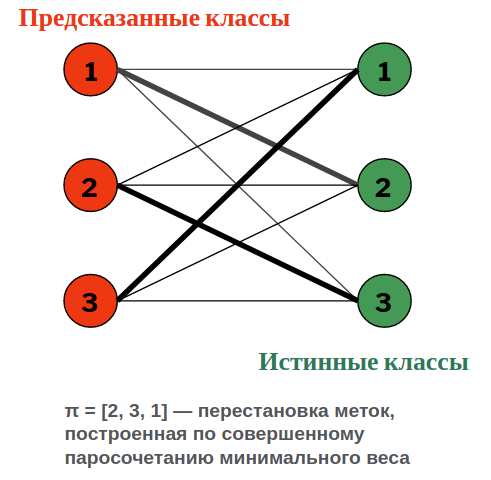
\includegraphics[keepaspectratio=true, scale=0.75]{images/label_permutation_reduction.png}
	\caption{Иллюстрация сведения задачи восстановления наиболее вероятной перестановки меток классов к поиску совершенного паросочетания минимального веса в двудольном графе. Веса — расстояния между столбцами матриц $\bm{P}$ и $\bm{Q}$, матриц предсказанных и истинных вероятностей клональных меток.} 
\end{figure}

\subsection{Заключительная версия XClone: BAF- и RDR-модули}
Текущая версия алгоритма XClone использует BAF и RDR для того, чтобы восстановить клональную структуру опухоли и определить профили ASCNV для каждого клона. Она лишена сразу нескольких недостатков прошлой версии:
\begin{itemize}
	\item не зависит от внешних алгоритмов детектирования CNV по данным single-cell секвенирования;
	\item для поиска оценки апостериорного максимума вместо медленного семплирования по Гиббсу используется эффективно автоматизированный вариационный байесовский вывод на GPU;
\end{itemize}
От пользователя требуется только предоставить BAM-файлы образцов и набор геномных позиций, использованных при секвенировании. Вся предобработка данных и дальнейшее обучение модели релизовано в виде отдельных скриптов с консольным интерфейсом, для использования которых достаточно задать пути к данным. 

Сам алгоритм принимает на вход три матрицы:
\begin{itemize}
	\item $\bm{RD}$ — матрица прочтений;
	\item $\bm{DP}$ — матрица прочтений, которые выравниваются на последовательности, содержащие хотя бы один ОНП;
	\item $\bm{AD}$ — матрица тех прочтений из $\bm{DP}$, которые выравниваются на материнский аллель;
\end{itemize}

Все три матрицы принадлежат $\N^{N \times M}$, где $N$ это число блоков после предобработки из раздела \ref{bin_linkage_em}, а $M$ — число клеток образца. Все три матрицы должны быть подсчитаны по данным scDNA-seq.

Также на вход алгоритма подаётся $K$  — ожидаемое число клональных линий в образце — и $\tau$, набор допустимых ASCNV $ \{c_{t}\}_{t=1}^{T} $, где $ c_{t} := (c_{t,m}, c_{t,p})$, где $c_{t,m}$ — число копий на материнской хромосоме, а $ с_{t, p} $ — соответственно, на отцовской. По умолчанию для $\tau$ содержит следующие 16 состояний:
\begin{align*}
	(&[0,0], [0,1], [0,2], [0,3],\\
	&[1,0], [1,1], [1,2], [1,3],\\ 
	&[2,0], [2,1], [2,2], [2,3],\\
	&[3,0], [3,1], [3,2], [3,3])
\end{align*}
BAF- и RDR-модули связаны скрытыми переменными $\bm{Z}, \bm{Y}$:
\begin{itemize}
	\item $z_{j,k} := I\{ \text{клетка } j \text{ принадлежит клональной линии } k \}$;
	\item $y_{i,k,t} := I\{ \text{блок } i \text{ в клональной линии } k \text{ находится в состоянии } c_{t} \} $;
\end{itemize}
на которых заданы априорные вероятности $\bm{\pi}, \bm{U}$:
\begin{equation}
	\begin{split}
		p(z_{j,k} = 1\ |\ \bm{\pi}) & = \mathtt{Multinom}(1; \bm\pi_{j}) = \pi_{j,k} \\
		p(y_{i,k,t} = 1\ |\ \bm{U}) & = \mathtt{Multinom}(1; \bm{u}_{i,k}) = u_{i,k,t} 
	\end{split}
	\label{Eq:xclone_vb_shared_priors}
\end{equation}

\subsubsection{Структура BAF-модуля}
Если блок $i$ в клетке $j$ находится в состоянии $c_{t}$, то $a_{i,j}$ подчиняется биномиальной модели с параметром $\theta_{i,t} \sim \mathrm{Beta}(\alpha_t, \beta_t)$, где $\alpha_t, \beta_t$ — параметры априорного распределения. Они одни и те же для всех блоков в состоянии $c_{t}$ и полагаются равными $\alpha_t = (c_{t,1} + 0.01)$ и $\beta_t = (c_{t,2} + 0.01)$. В формульной записи:

\begin{equation}
	p(a_{i,j}\ |\ d_{i,j}, \theta_{i, t}) = \mathtt{Binom}(a_{i,j}\ |\ d_{i,j}, \theta_{i,t}).
	\label{Eq:xclone_vb_ase_base}
\end{equation}

где $a_{i, j}, d_{i, j}$ — элементы матриц $\bm{AD}, \bm{DP}$ на позиции $(i, j)$. В предположении, что числа прочтений в соседних блоках независимы, функция правдоподобия записывается следующим образом:

\begin{equation}
	p(A, D | Z, Y, \bm\theta)  = \prod_{i=1}^{N} \prod_{j=1}^{M} \prod_{k=1}^{K}\prod_{t=1}^{T} p(a_{i,j}\ |\ d_{i,j}, \theta_{i,t}) ^{z_{j,k} \times y_{i,k,t}}
	\label{Eq:xclone_vb_ase_lik}
\end{equation}

\subsubsection{Структура RDR-модуля}
Для каждой клональной линии $k$ модель числа прочтений задаётся мультиномиальным распределением. Каждому блоку $i$ в этой модели назначается вероятность $f_{i,k}$. Она задаётся формулой
\begin{equation}
	\begin{aligned}
		f_{i,k} &:= \dfrac{\sum_{t=1}^{T} m_i \exp[\gamma_t] P(y_{i,k,t}=1)}{\sum_{b=1}^{N}\sum_{t=1}^{T} m_b \exp[\gamma_t] P(y_{b,k,t}=1)}
	\end{aligned}
\label{Eq:xclone_vb_rdr_multinomial_def}
\end{equation}
Где $m_{i}$ — доля прочтений, попадающих в блок $i$ в здоровой клетке при стремлении глубины покрытия к бесконечности (или какая-то оценка этой величины), $\exp\{\gamma_t\}$ — амплификация, вызванная наличием $c_{t,m} + c_{t,p}$ копий блока в геноме (здесь возведение в степень нужно для того, чтобы гарантировать неотрицательность). Эта модель согласуется с теорией для данных scDNA-seq, т.к. после коррекции технических факторов для ДНК-секвенирования правомерны предположения о том, что прочтения распределяются по геному равномерно, а систематические отклонения от этого правила могут быть вызваны только loss- или gain-событиями (см. модель ДНК-секвенирования из раздела \ref{dna_seq_probabilistic_model}). 

Тогда функция правдоподобия запишется как
\begin{equation}
	\begin{aligned}
		\bm r_{j} &:= (r_{1, j}, \ldots, r_{N, j})\\
		p(\bm r_{j}\ | \bm f_{k}) &:= \mathtt{Multinom}\left (\bm r_{j}\ \middle|\ \sum_{i=1}^{N} r_{i,j}, \bm f_{k}\right )\\
		p(\bm{RD}\ |\ \bm{Z}, \bm{Y}, \bm{m}, \bm{\gamma})  & := \prod_{j=1}^{M} \prod_{k=1}^{K} p\left (\bm r_{j}\ \middle|\ \sum_{i=1}^{N} r_{i,j}, \bm f_{k}\right ) ^{z_{j,k}}
	\end{aligned}
	\label{Eq:xclone_vb_rdr_lik}
\end{equation}

Если $\bm{m}$ заранее неизвестно, то его можно смоделировать посредством задания априорного распределения $\mathtt{Dirichlet}(\bm\omega)$. Аналогично для $\mathbf{\gamma}$ в качестве априорного распределения задаётся $\mathtt{GP}(\bm\mu, \bm\Sigma)$, где под $\mathtt{GP}$ подразумевается дискретный гауссовский процесс с $\mu_t := \log((c_{t,m} + c_{t,p}) / 2 + \varepsilon)$ для достаточного малого положительного $\varepsilon$, а матрица ковариаций $\bm\Sigma$ задаётся RBF-ядром $K(\bm c_t, \bm c_{t\prime}) := l_1 \exp\{-l_2[(c_{t,m}-c_{t\prime,m})^2 + (c_{t,p}-c_{t\prime,p})^2]\}$, где $l_1,\ l_2$ — гиперпараметры модели. В формульной записи:
\begin{equation}
	\begin{split}
		\bm m\ |\ \bm \omega &\sim \mathtt{Dirichlet}( \bm\omega)\\
		\bm \gamma\ |\ \bm\mu, \Sigma &\sim \mathtt{\mathtt{GP}}(\bm\mu, \bm\Sigma) \\
	\end{split}
	\label{Eq:xclone_vb_rdr_priors}
\end{equation}

\subsubsection{Вариационный байесовский вывод}
\paragraph{Общее описание метода}$  $\\
Пусть $\bm{X} = (X_1, \ldots, X_n)$ — выборка из распределения с плотностью $p_{\theta}(\bm{X})$ ($p_{\theta}(\bm{X}) = \prod_{i=1}^{n} p_{\theta}(X_i)$), где $\theta$ — набор параметров распределения. Пусть $q$ — априорное распределение на $\Theta$ — множестве допустимых параметров. Тогда $f(\theta, \bm{X}) := p_{\theta}(\bm{X}) q(\theta)$ — плотность совместного распределения на $\Theta \times \mathcal{X}$. Тогда апостериорная плотность на параметрах выражается как
$$
	q(\theta\ |\ \bm{X}) := \frac{f(\theta, \bm{X})}{p(\bm{X})} = \frac{f(\theta, \bm{X})}{\int_{\Theta} f(t, \bm{X}) dt }  = \frac{f(\theta, \bm{X})}{\int_{\Theta} p_{t}(\bm{X}) q(t) dt } 
$$
Величину $p(\bm{X})$ в знаменателе называют \textbf{обоснованностью}. В общем случае она не выражается в аналитических функциях. 

Пусть стоит задача найти оценку апостериорного максимума (ОАМ) — $\arg\max\limits_{\Theta} q(\theta\ |\ \bm{X})$, — а также распределение на всех параметрах из $\theta$. В силу того, обоснованность $p(\bm{X})$ это константа, можно максимизировать не $q(\theta \|\ \bm{X})$, а $f(\theta, \bm{X})$. Но совместная плотность как функция может быть устроена произвольно сложно. Уже при счётном $\Theta$ поиск её максимума это нетривиальная задача. Тем не менее, задача поиска ОАМ допускает альтернативную формулировку в форме задачи непрерывной оптимизации.

\begin{definition}[\textit{KL-дивергенция}]
	Пусть $p, q$ — плотности распределений $P, Q$ над одним вероятностным пространством $(\Omega, \mathcal{F}, \P)$. Тогда KL-дивергенцией $KL(P\ \|\ Q)$ называют величину $ \int_{\Omega} p(x) \log \frac{p(x)}{q(x)} dx $.
\end{definition}

\begin{claim}
	Пусть $\mathbb{F}_{\mathcal{X}}$ — пространство абсолютно непрерывных распределений над вероятностным пространством $\mathcal{X} = (\Omega, \mathcal{F}, \P)$, тогда
	\begin{enumerate}
		\item $\forall P, Q \in \mathbb{F}_{\mathcal{X}}: KL(P\ \|\ Q) \ge 0$, причём $KL(P\ \|\ Q) = 0 \iff P \overset{\text{п.вс.}}{=} Q$.
		\item $\forall P_1, P2, Q \in \mathbb{F}_{\mathcal{X}}: KL(P_1\ \|\ P_2) \le  KL(P_1\ \|\ Q) + KL(Q\ \|\ P_2)$
	\end{enumerate}
	Кроме того, для произвольного $\mathcal{X}$ могут найтись $ P, Q \in \mathbb{F}_{\mathcal{X}}$, такие что $KL(P\ \|\ Q) \neq KL(Q\ \|\ P) $, что не позволяет считать KL-дивергенцию метрикой на на $\mathbb{F}_{\mathcal{X}}$.
\end{claim} 

Вариационный байесовский вывод (далее — VB) основан на следующей идее: заменить апостериорное распределение $Q(\theta\ |\ \bm{X})$, которое может быть устроено сколь угодно сложно, на удобную для оптимизации аппроксимацию $ Q^{\ast}(\theta) $ из семейства распределений $\mathcal{Q}$. Тогда есть следующий алгоритм приближённого поиска ОМА:

\begin{algorithm}[H]
	\SetAlgoLined
	\KwResult{$\theta^{\ast}_{0}, Q^{\ast}_{0}$ — приближение ОМА и соотв. аппроксимация }
	$Q^{\ast}_{0} := \arg\min\limits_{Q^{\ast} \in \mathcal{Q}} KL(Q^{\ast}\ \|\ Q(\cdot\ |\ \bm{X})) $\;
	$\theta^{\ast}_{0} := \arg\max\limits_{\theta \in \Theta} Q^{\ast}_{0}(\theta) $
	\caption{Вариационный байесовский вывод, общий вид}
\end{algorithm}

Этот метод центральный для алгоритма XClone, потому в этом разделе приведен его подробный обзор.
\begin{definition}[\textit{ELBO}]
	В обозначениях данного раздела, величину 
	$$
	\mathcal{L}(Q^{\ast}) := \int_{\Theta} q^{\ast} (\theta) \log \frac{f(\theta, \bm{X})}{q^{\ast}(\theta)} d\theta
	$$
	называют ELBO — evidence lower bound. На русский язык это можно перевести как <<нижняя оценка логарифма обоснованности>>, но устоявшегося перевода в сообществе нет, потому обычно используют сокращение ELBO.
\end{definition}

\begin{claim}
	Максимизация ELBO по $Q^{\ast} \in \mathcal{Q}$  эквивалентна минимизации $KL(Q^{\ast}\ \|\ Q_{\bm{X}})$, где $Q_{\bm{X}}(\theta)Q(\cdot\ |\ \bm{X})$.
\end{claim}
\begin{proof}
	Распишем $KL(Q^{\ast}\ \|\ Q_{\bm{X}})$:
	\begin{equation}
	\begin{aligned}
	KL(Q^{\ast}\ \|\ Q_{\bm{X}}) &= \E_{\phi \sim Q^{\ast}} \log \frac{q^{\ast}(\phi)}{q_{\bm{X}}(\phi)} =\\
	&= -\E_{\phi \sim Q^{\ast}} \log \frac{q_{\bm{X}}(\phi)}{q^{\ast}(\phi)} =\\
	&= -\E_{\phi \sim Q^{\ast}} \log \frac{f(\phi, \bm{X})}{p(\bm{X}) q^{\ast}(\phi)} =\\
	&= -\E_{\phi \sim Q^{\ast}} \log \frac{f(\phi, \bm{X})}{q^{\ast}(\phi)} + \E_{\phi \sim Q^{\ast}} \log  p(\bm{X}) =\\
	&= -\mathcal{L}(Q^{\ast}) + \log p(\bm{X}) 
	\end{aligned}
	\label{ELBO_derivation}
	\end{equation}
	Отсюда получаем, что $ \log p(\bm{X}) = L(Q^{\ast}) + KL(Q^{\ast}\ \|\ Q_{\bm{X}}) $. Логарифм обоснованности не зависит от $\theta$, потому максимизация $\mathcal{L}(Q^{\ast})$ эквивалентна минимизации $ KL(Q^{\ast}\ \|\ Q_{\bm{X}}) $, а потому и решению задачи вариационного байесовского вывода.
	
	ELBO можно получить и иначе, расписав $\log p(\bm{X})$:
	\begin{equation}
		\begin{aligned}
			\log p(\bm{X}) &= \log \int_{\Theta} f(\theta, \bm{X}) d\theta \\
			&= \log \int_{\Theta} f(\theta, \bm{X}) \frac{q^{\ast}(\theta)}{q^{\ast}(\theta)} d\theta =\\
			&= \log \E_{\phi \sim Q^{\ast}} \frac{f(\phi, \bm{X})}{q^{\ast}(\phi)} =\\
			&= \left[ \text{Неравенство Йенсена} \right] \ge\\
			&\ge \E_{\phi \sim Q^{\ast}} \log \frac{f(\phi, \bm{X})}{q^{\ast}(\phi)} = \mathcal{L}(Q^{\ast})
			\end{aligned}
		\label{alternative_ELBO_derivation}
	\end{equation}
	Такое доказательство не проясняет связь с VB, но полезно в контексте других приложений и помогает понять, почему эта величина имеет именно такое название.
\end{proof}

\begin{remark}
	В силу того, что KL-дивергенция не симметрична, вид оптимальной аппроксимации может противоречить интуитивному представлению о том, как она должна быть устроена. Для лучшего понимания полезно рассмотреть несколько примеров из \cite{MurphyProbabilisticML} (стр. 734), которые иллюстрируют разницу между $KL(Q^{\ast}\ \|\ Q_{\bm{X}})$ — \textit{forward KL} — и $KL(Q_{\bm{X}}\ \|\ Q^{\ast})$ — \textit{reverse KL}. 
	
	\begin{figure}[H]
		\centering
		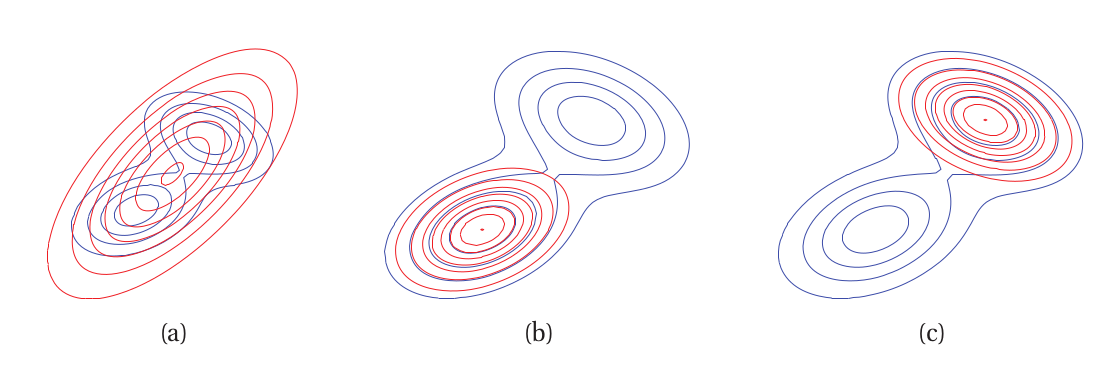
\includegraphics[keepaspectratio=true, scale=0.4]{images/forward_reverse_kl_bimodal.png}
		\caption{Аппроксимация бимодального распределения $Q$ (синие линии) двумерным гауссовским распределением $Q^{\ast}$ (красные линии). (а) — результат минимизации $KL(Q\ \|\ Q^{\ast})$, (b)-(с) — варианты оптимального приближения при минимизации $KL(Q^{\ast}\ \|\ Q)$ } 
	\end{figure}
	
	\begin{figure}[H]
		\centering
		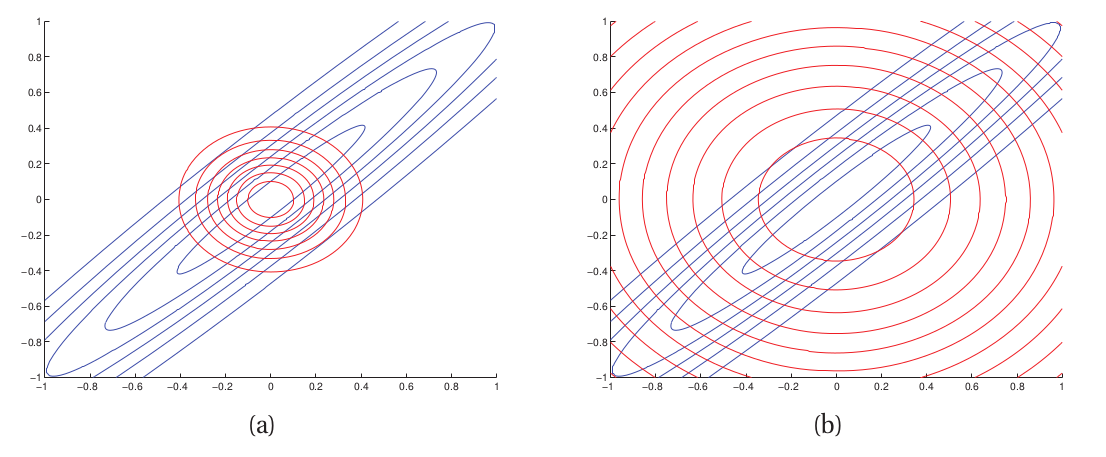
\includegraphics[keepaspectratio=true, scale=0.4]{images/forward_reverse_kl_symmetric_gaussian.png}
		\caption{Аппроксимация распределения $Q$ симметричным двумерным гауссовским распределением $Q^{\ast}$. (а) — результат минимизации $KL(Q^{\ast}\ \|\ Q)$, (b) — $KL(Q\ \|\ Q^{\ast})$} 
	\end{figure}
	
	Видно, что при минимизации reverse-KL локальные максимумы аппроксимации $Q^{\ast}$ скорее всего будут совпадать с таковыми у $Q$. При этом может быть так, что $Q^{\ast}$ будет хорошо приближать $Q$ только на каком-то множестве, которому распределение $Q$ сопоставляет большую вероятность, потому её называют \textbf{zero-forcing}. Минимизация же forward KL будет стремиться хорошо объяснить всё распределение $Q$ в целом, а не только отдельные, важные фрагменты, её называют \textbf{zero-avoiding}.  В обоих случаях наблюдаемое поведение связано с тем, какая плотность оказывается в знаменателе отношения под логарифмом.	
\end{remark}

Указанная в предыдущем замечании особенность \textbf{очень важная}. Она показывает, что VB, в отличие от MCMC, может даже в пределе не давать возможности семплировать из истинного распределения. Тем не менее, VB существенно проще вычислительно, так как это оптимизационная задача, для решения которой есть хорошо разработанные методы стохастической и распределённой оптимизации. Более того, часто одного только VB бывает достаточно. Вопрос о том, когда использовать VB, а когда MCMC, хорошо резюмирует приведенная цитата из \cite{VariationalInferenceReview}:

\textit{<<Thus, variational inference is suited to large data sets and scenarios where we want to
	quickly explore many models; MCMC is suited to smaller data sets and scenarios where
	we happily pay a heavier computational cost for more precise samples. For example, we
	might use MCMC in a setting where we spent 20 years collecting a small but expensive data
	set, where we are confident that our model is appropriate, and where we require precise
	inferences. We might use variational inference when fitting a probabilistic model of text to
	one billion text documents and where the inferences will be used to serve search results
	to a large population of users. In this scenario, we can use distributed computation and
	stochastic optimization to scale and speed up inference, and we can easily explore many
	different models of the data.>>}

\begin{remark}
	ELBO можно переписать как $\mathcal{L}(Q^{\ast}) = \E_{\phi \sim Q^{\ast}} f(\phi, \bm{X}) - H(Q^{\ast})$, где $H$ — энтропия. Если $Q^{\ast} = Q_{\bm{X}}$, то левое слагаемое это в точности величина, которая максимизируется на M-шаге EM-алгоритма. Это сходство неслучайно и поясняется в \cite{VariationalInferenceReview}:
	\textit{<<Unlike variational inference, EM assumes the expectation over posterior distribution of latent variables is computable and uses it in otherwise difficult parameter estimation problems. Unlike EM, variational inference does not estimate fixed model parameters — it is often used in a Bayesian setting where classical parameters are treated as latent variables. Variational inference applies to models where we cannot compute the exact conditional of the latent variables.>>}
\end{remark}

Чаще всего $\mathcal{Q}$ выбирают таким, чтобы распределения из него факторизуются по параметрам, т.е. что 
$$
	q^{\ast}(\theta) = \prod_{i=1}^{m} q_{i}^{\ast}(\theta_i)
$$
где $m$ это число параметров. Это т.н. \textbf{mean field approximation} — метод, вдохновлённый т.н. моделью Изинга из статистической физики. В \cite{VariationalInferenceReview} (стр. 9-10) описан эффективный алгоритм оптимизации маржинальных плотностей $q_{i}^{\ast}$. Тем не менее, в модели XClone он не используется, т.к. максимизация ELBO происходит автоматически за счёт использования примитивов из Tensorflow.Distributions\cite{TensorflowDistributions}. При этом $\mathcal{L}(Q^{\ast})$ оптимизируется неявно, посредством максимизации правой части равенства $\mathcal{L}(Q^{\ast}) = KL(Q^{\ast}\ \|\ Q) + \log p(\bm{X})$, т.к. использование сопряжённых распределений позволяет расписать её в пригодном для покоординатной оптимизации виде.

\paragraph{VB в алгоритме XClone}$ $\\
Апостериорные распределения на параметрах модели XClone имеют вид
\begin{equation}
	\begin{split}
		&p(\bm{Z}, \bm{Y}, \bm{\theta}, \bm{m}, \bm{\gamma}\ |\ \bm{AD}, \bm{DP}, \bm{RD}) \propto\\ 
		&\propto p(\bm{Z}, \bm{Y}, \bm{\theta}, \bm{m}, \bm\gamma) p(\bm{AD}, \bm{DP}, \bm{RD} | \bm{Z}, \bm{Y}, \bm{\theta}, \bm{m}, \bm{\gamma}) = \\
		& = p(\bm{Z}, \bm{Y}, \bm{\theta}, \bm{m}, \bm{\gamma}) \cdot \mathunderline{green}{p(\bm{AD}, \bm{DP} | \bm{Z}, \bm{Y}, \bm{\theta})} \cdot \mathunderline{red}{p(\bm{RD}\ |\ \bm{Z}, \bm{Y}, \bm{m}, \bm{\gamma})}
	\end{split}
	\label{Eq:xclone_vb_posterior}
\end{equation}
где функция правдоподобия распадается в произведение по BAF- и RDR-модулям, т.к. матрицу $\bm{RD}$ можно по смыслу считать независищяей от матриц $\bm{AD}, \bm{DP}$ по смыслу. Строго говоря, между $\bm{DP}$ и $\bm{RD}$ есть положительная корреляция, но она не добавляет новой информации в модель, потому ею было решено пренебречь. Скрытые переменные из $\Omega := \{\bm{Z}, \bm{Y}, \bm{m}, \bm{\gamma}\}$ независимы в совокупности. Апостериорное распределенияе $p(\Omega\ |\ \bm{AD}, \bm{DP}, \bm{RD})$, как следствие, факторизуется по скрытым переменным. В силу того, что в модели всюду используются сопряжённые распределения, апостериорное распределение имеет тот же вид, что и априорное. Тем не менее, явно вычислить его параметры затруднительно, проще выразить VB через примитивы Tensorflow.Distributions\cite{TensorflowDistributions} и найти ОАМ стохастическим градиентным спуском в пространстве параметров.

Стоит отметить, что ELBO в стат.модели XClone по явной формуле (через матожидание) оптимизировать сложнее, чем его представление через разность логарифма обоснованности и KL-дивергенции.  
\begin{equation}
	\mathtt{L}(q) = \int{ q(\Omega) \log p(\bm{AD}, \bm{DP}, \bm{RD}\ |\ \Omega)} \text{d} \Omega -\mathtt{KL}(q(\Omega)\ \|\ p(\Omega))
\end{equation}

\noindent Логарифм обоснованности распадается в сумму по BAF- и RDR-модулям.
\begin{equation} 
	\begin{split}
		&\int{ q(\Omega) \log p(\bm{AD}, \bm{DP}, \bm{RD}\ |\ \Omega)} \text{d} \Omega =\\
		&= \mathunderline{green}{\int{ q(\bm{Z}, \bm{Y}, \bm{\theta}) \log p(\bm{AD}, \bm{DP}\ |\ \bm{Z}, \bm{Y}, \bm{\theta})} \text{d} \bm Z \text{d} \bm{Y} \text{d} \bm{\theta}} + \\
		& + \mathunderline{red}{\int{ q(\bm{Z}, \bm{Y}, \bm{m}, \bm{\gamma}) \log p(\bm{RD}\ |\ \bm{Z}, \bm{Y}, \bm{m}, \bm{\gamma})} \text{d} \bm{m} \text{d} \bm{\gamma}}
	\end{split}
\end{equation}

\paragraph{Вывод ELBO для BAF-модуля}$  $\\
\begin{claim}
Лог-боснованность BAF-модуля можно расписать как:
\begin{equation}
	\footnotesize
	\begin{split}
		&\mathunderline{green}{\mathbb{E}_{\bm{Z}, \bm{Y}, \bm{\theta}}\log p(\bm{AD}, \bm{DP}\ |\ \bm{Z}, \bm{Y},\bm{\theta})} = \\
		& = \int{ q(\bm{Z}, \bm{Y}, \bm{\theta}) \log p(\bm{AD}, \bm{DP}\ |\ \bm{Z}, \bm{Y}, \bm\theta)} \text{d} \bm{Z} \text{d} \bm{Y} \text{d} \bm{\theta} \\ 
		& = \sum_{i=1}^N \sum_{j=1}^M  \sum_{k=1}^K  \sum_{t=1}^T  \left\{\tilde \pi_{j,k} \tilde u_{i,k,t}  [w_{i,j} + a_{i,j}\psi(\tilde \alpha_t) + b_{i,j}\psi(\tilde \beta_t) - d_{i,j}\psi(\tilde \alpha_t + \tilde \beta_t) ]  \right\}
	\end{split}
\end{equation}
где $b_{i,j} := d_{i,j} - a_{i,j}$, $\tilde \cdot$ указывает, что имеется в виду аппроксимация истинной апостериорной вероятности, $w_{i,j} := \log \binom{d_{i,j}}{a_{i,j}}$, $\psi(\cdot)$ — дигамма-функция, $\psi(z) := \frac{\Gamma'(z)}{\Gamma(z)} = -\gamma + \int_{0}^{1} \left( \frac{1 - t^{z}}{1 - t} \right) dt$, где $\Gamma$ это гамма-функция Эйлера, а $\gamma$ это константа Эйлера-Маскерони, $\gamma := \lim\limits_{n \to \infty} \left( -\ln n  + \sum_{k=1}^{n} \frac{1}{k} \right)$.
\end{claim}
\begin{proof}
	BAF-модуль эквивалентен модели \cite{Vireo} и имеет аналогичное доказательство.
	\begin{equation*}
		\footnotesize
		\begin{split}
			& \int{ q(\bm{Z}, \bm{Y}, \bm{\theta}) \log p(\bm{AD}, \bm{DP}\ |\ \bm{Z}, \bm{Y}, \bm{\theta})} \text{d} \bm{Z} \text{d} \bm{Y} \text{d} \bm{\theta} \\ 
			& = \mathbb{E}_{\bm{Z}, \bm{Y}, \bm{\theta}}\left[\log p(\bm{AD}, \bm{DP}\ |\ \bm{Z}, \bm{Y}, \bm{\theta})\right] \\
			& = \mathbb{E}_{\bm{Z}, \bm{Y}, \bm{\theta}}\left[\log \prod_{i=1}^{N} \prod_{j=1}^{M} \prod_{k=1}^{K}\prod_{t=1}^{T} p(a_{i,j}\ |\ d_{i,j}, \theta_t) ^{z_{j,k} \times y_{i,k,t}}\right] \\
			& = \mathbb{E}_{\bm{Z}, \bm{Y}, \bm\theta}\sum_{i=1}^{N} \sum_{j=1}^{M} \sum_{k=1}^{K}\sum_{t=1}^{T} [{z_{j,k} y_{i,k,t} \log{\mathtt{Binom}(a_{i,j}\ |\ d_{i,j}, \theta_t)}}] \\
			& = \sum_{i=1}^{N} \sum_{j=1}^{M} \sum_{k=1}^{K}\sum_{t=1}^{T} \mathbb{E}_{\bm{Z}, \bm{Y}, \bm\theta}[z_{j,k} y_{i,k,t} \log{\mathtt{Binom}(a_{i,j}\ |\ d_{i,j}, \theta_t)}] \\
			& = \sum_{i=1}^{N} \sum_{j=1}^{M} \sum_{k=1}^{K}\sum_{t=1}^{T} \mathbb{\bm{E}}_{\bm{Z}}[z_{j,k}] \mathbb{E}_{\bm{Y}}[y_{i,k,t}] \mathbb{E}_{\bm\theta}[\log{\mathtt{Binom}(a_{i,j}\ |\ d_{i,j}, \theta_t)}] \\
			& = \sum_{i=1}^{N} \sum_{j=1}^{M} \sum_{k=1}^{K}\sum_{t=1}^{T} \left\{ \tilde \pi_{j,k} \tilde u_{i,k,t} \mathbb{E}_{\bm\theta}[\log{\mathtt{Binom}(a_{i,j}\ |\ d_{i,j}, \theta_t)}]\right\} \\
			& = \sum_{i=1}^N \sum_{j=1}^M  \sum_{k=1}^K  \sum_{t=1}^T  \left\{ \tilde \pi_{j,k} \tilde u_{i,k,t}  [w_{i,j} + a_{i,j}\psi(\tilde\alpha_t) + b_{i,j}\psi(\tilde\beta_t) - d_{i,j}\psi(\tilde\alpha_t + \tilde\beta_t) ]  \right\}
		\end{split}
	\end{equation*}
	Где матожидание логарифма плотности бета-биномиального распределения, имеет следующие представление, задействующее дигамма-функцию:
	\begin{align*}
			& \mathbb{E}_{\alpha, \beta}[\log{q(a\ |\ d, \theta)}] = \\
			& = \mathbb{E}_{\alpha, \beta}[\log{\mathtt{Binom}(a; d, \theta)}] = \\
			& = \mathbb{E}_{\alpha, \beta}\left[\log{\binom{a}{d}} + a\log{\theta} + (d-a)\log{(1-\theta)}\right] = \\
			& = \log{\binom{a}{d}} + a\mathbb{E}_{\theta}[\log{\theta}] + (d-a)\mathbb{E}_{\beta, \alpha}[\log{(1-\theta)}] = \\
			& = \log{\binom{a}{d}} + a(\psi(\alpha) - \psi(\alpha + \beta)) + (d-a) (\psi(\beta) - \psi(\alpha + \beta)) = \\
			& = \log{\binom{a}{d}} + a\psi(\alpha) + (d-a)\psi(\beta) - d \psi(\alpha + \beta)
	\end{align*}
	Где тождество $\mathbb{E}_{\alpha, \beta}[\log{\theta}] = \psi(\alpha) - \psi(\alpha + \beta)$ доказывается так:
	\begin{align*}
			\mathbb{E}_{\alpha, \beta} \log \theta =
			&= \int_0^1 \ln x\, \mathtt{Beta}(x; \alpha, \beta) dx =\\ 
			&= \int_0^1 \ln x \,\frac{ x^{\alpha-1}(1-x)^{\beta-1}}{\mathtt{B}(\alpha,\beta)} dx =\\
			&= \frac{1}{\mathtt{B}(\alpha,\beta)} \, \int_0^1 \frac{\partial x^{\alpha-1}(1-x)^{\beta-1}}{\partial \alpha} dx =\\
			&= \frac{1}{\mathtt{B}(\alpha,\beta)} \frac{\partial}{\partial \alpha} \int_0^1 x^{\alpha-1}(1-x)^{\beta-1} dx =\\
			&= \frac{1}{\mathtt{B}(\alpha,\beta)} \frac{\partial \mathtt{Beta}(\alpha,\beta)}{\partial \alpha} dx = \\
			&= \frac{\partial \ln \mathtt{B}(\alpha,\beta)}{\partial \alpha} = \\
			&= \frac{\text{d} \ln \Gamma(\alpha)}{\text{d}\alpha} - \frac{\partial \ln \Gamma(\alpha + \beta)}{\partial \alpha} = \\
			&= \psi(\alpha) - \psi(\alpha + \beta)
	\end{align*}
\end{proof}

\begin{remark}
	Отдельный интерес представляет подход к вычислению величины $w_{i,j} = \log \binom{d_{i,j}}{a_{i,j}}$. Дело в том, что числа с плавающей точкой в реализации большинства языков программирования имеют ограниченную точность, которая не позволяет отдельно вычислить биномиальный коэффициент, а потом взять от него логарифм. Даже в языке Python, в котором реализована длинная арифметика в целых числах, взятие логарифма может привести к переполнению типа при больших значениях $d_{i, j}$ и $a_{i, j} \simeq \frac{1}{2} d_{i, j}$. 
	
	Безусловно, можно вычислять $\log \binom{d_{i,j}}{a_{i,j}}$ как 
	$$
		\sum_{s=0}^{a_{i, j} - 1} \log (d_{i,j} - s)  - \sum_{s=0}^{a_{i, j}} \log s
	$$ 
	Тем не менее, при большой разнице между $d_{i, j}$ и $a_{i, j}$ при таком подходе ошибки представления логарифмов накапливаются, что может привести к заметному расхождению подсчитанной величины с истинным значением. 
	
	Этих недостатков лишена красивая аппроксимация величины $\log n!$, полученная логарифмированием асимптотической формулы для $n!$, полученной великим математиком Сринивасой Рамануджаном\cite{RamanujanLostNotebook} и уточняющей формулу Стирлинга. 
	$$
		\log n! \simeq n \log n - n  + \frac{\log (n (1 + 4n (1 + 2n)))}{6} + \frac{\log \pi}{2}
	$$
	Именно эта формула используется при вычислении $w_{i,j}$ в алгоритме XClone.
\end{remark}

\paragraph{Вывод ELBO для RDR-модуля}$  $\\
\begin{claim} \label{claim:rdr_evidence_mc}
	Лог-обоснованность RDR-модуля можно записать как
	\begin{equation}
		\footnotesize
		\begin{aligned}
			&\mathunderline{red}{\E_{\bm{Z}, \bm{Y}, \bm{m}, \bm{\gamma}} \log p(\bm{RD}\ |\ \bm{Z}, \bm{Y},\bm{m}, \bm{\gamma})} =\\
			&= \int{ q(\bm{Z}, \bm{Y}, \bm{m}, \bm{\gamma}) \log p(\bm{RD}\ |\ \bm{Z}, \bm{Y},\bm{m}, \bm{\gamma})} \text{d} \bm{m}, \text{d} \bm{\gamma} =\\
			&= \sum_{i=1}^{N}\sum_{j=1}^{M}\sum_{k=1}^{K} \widetilde{\pi}_{j,k} \cdot r_{ij} \cdot \mathbb{E}_{\bm{m}, \bm{\gamma}} \log \widetilde{f}_{i,k} + C
		\end{aligned}
	\end{equation}
	где $\tilde \cdot$ указывает, что имеется в виду аппроксимация истинной апостериорной вероятности, а
	$$
		\widetilde{f}_{i,k}\ |\ \bm{m}, \bm{\gamma} := \dfrac{\sum_{t=1}^{T} m_i \exp[\gamma_t] \tilde u_{i,k,t}}{\sum_{b=1}^{N}\sum_{t=1}^{T} m_b \exp[\gamma_t] \tilde u_{b,k,t}}
	$$
\end{claim}
\begin{proof}
	\begin{align*}
		&\int{ q(\bm{Z}, \bm{Y}, \bm{m}, \bm{\gamma}) \log p(\bm{RD}\ |\ \bm{Z}, \bm{Y}, \bm{m}, \bm\gamma)} \text{d} \bm{m}, \text{d} \bm{\gamma} =\\
		&= \mathbb{E}_{\bm{Z}, \bm{Y}, \bm{m}, \bm{\gamma}} \log p(\bm{RD}\ |\ \bm{Z}, \bm{Y},\bm{m}, \bm{\gamma})  =\\
		&= \text{см. формулу } \ref{Eq:xclone_vb_rdr_lik} =\\
		&= \mathbb{E}_{\bm{Z}, \bm{Y}, \bm{m}, \bm \gamma} \left[ \sum_{j=1}^{M}\sum_{k=1}^{K} \log p\left(\bm r_{j}\ \middle|\ \sum_{i=1}^{N} r_{i,j}, \bm f_{k}\right)^{z_{j,k}} \right] =\\
		&= \sum_{j=1}^{M}\sum_{k=1}^{K} \mathbb{E}_{\bm{Z}, \bm{Y}, \bm{m}, \bm{\gamma}} \left[ z_{j,k} \cdot \log \left(r_{j}! \prod_{i=1}^{N}
		\frac{\widetilde{f}_{i,k}^{r_{i,j}}}{r_{i,j}!} \right) \right] =\\
		&= \text{ обозначим сумму всех констант через $C$ } =\\
		&= \sum_{i=1}^{N}\sum_{j=1}^{M}\sum_{k=1}^{K} \mathbb{E}_{\bm{Z}, \bm{Y}, \bm{m}, \bm{\gamma}} \left[ z_{j,k} \cdot r_{ij} \log \widetilde{f}_{i,k}\right] + C =\\
		&= \sum_{i=1}^{N}\sum_{j=1}^{M}\sum_{k=1}^{K} \widetilde{\pi}_{j,k} \cdot r_{ij} \cdot \mathbb{E}_{\bm{m}, \bm \gamma} \log \widetilde{f}_{i,k} + C
	\end{align*}
\end{proof}

\subsubsection{Известные недостатки и планы по их исправлению}
\paragraph{Избыточная сложность исходной модели}$  $\\
Эксперименты показали, что модель можно упростить: 
\begin{itemize}
	\item В коде XClone $\bm{m}$ фиксировано и выводится из теоретических соображений о равномерном распределении прочтений по геному. Т.е. $m_{i} = \frac{l_i}{\sum_{b=1}^{N} l_b}$ это достаточно хорошая оценка матожидания доли прочтений в сегменте $i$, где $l_i$ это длина $i$-го блока в сегментации.
	\item Далее, среднее значение $\bm{\gamma}$ тоже фиксировано, $\E \gamma_t := \log \frac{c_{t,m} + c_{m, 2}}{2} - \frac{e^{l_1^2}}{2}$, благодаря чему $ \E \exp(\gamma_t) = \frac{c_{t,m} + c_{m, 2}}{2} $, где $l_1$ это гиперпараметр ковариационной функции гауссовского процесса $\bm{\gamma}$. По изначальной задумке, по которой XClone можно было применять и для scRNA-seq данных, переменное $\bm{\gamma}$ было нужно для того, чтобы учесть не связанные с числом копий причины аллельного-дисбаланса в транскриптомных данных. 
	
	После того, как стало ясно, что транскриптомные данные этой же моделью обработать не получится из-за шумного BAF-сигнала и более сложной природы RDR-сигнала (в силу разреженности данных), потребность в переменном $\bm{\gamma}$ отпала. Более того, в силу того, что соотв. KL-слагаемое давало несущественный вклад в функцию ошибки, распределение на $\bm{\gamma}$ буквально за несколько итераций  вырождалось и теряло содержательный смысл. 
	\begin{figure}[H]
		\centering
		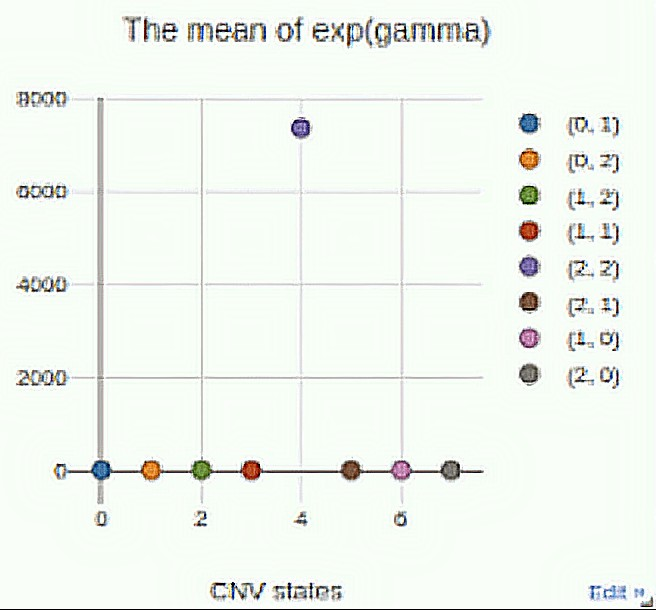
\includegraphics[keepaspectratio=true, scale=0.4]{images/amplfication_factors_posterior_collapse.jpeg}
		\caption{Вырождение апостериорного распределения. Ось Ох — координаты, ось Оу — матожидание вдоль компоненты. До того, как было принято решение зафиксировать $\gamma_t$, распределение на $\bm{\gamma}$ буквально за пару итераций VB вырождалось в одномерное.}
	\end{figure}
	Такое поведение можно было подавить умножением соотв. KL-слагаемого на большой множитель (порядка $10^6$), но такое преобразование было лишено смысла.
	\item Аналогично, связь между BAF- и RDR-модулями через $\bm{Z}$ и $\bm{Y}$ оказалась слишком слабой. Из-за этого получалась абсурдная ситуация, когда BAF-модуль выводил правильные $\theta$, но они были никак не согласованы с ASCNV, которые выводил RDR-модуль. Как следствие было решено избавиться от первой размерности: $\forall i, j\ \forall t: \theta_{i,t} \stackrel{d}{=} \theta_{j, t},\ \E \theta_{i, t} = \frac{c_{t, m}}{c_{t, m} + c_{t, p}} $, где $\stackrel{d}{=}$ означает равенство по распределению, и зафиксировать параметры $\alpha_t$ и $\beta_t$. 
	
	В самом деле, блок-зависимые BAF-ы имели смысл для транскриптомных данных, где картина экспрессии зависела от состояния клетки в момент секвенирования, что искажало сигнал аллельного дисбаланса. После того, как стало ясно, что VB будет применяться только к геномным данным, потребность в блок-специфичных BAF-ах отпала сама собой.
	
	Более того, невооружённым взглядом видно, что BAF-модуль гораздо проще, чем RDR-модуль. Более того, гетерозиготные ОНП составляют малую долю от всего генома, и примерно половины прочтений теряется при переходе от $\bm{RD}$ к $\bm{DP}$. Как следствие, обоснованность RDR-модуля была на несколько порядков больше обоснованности BAF-модуля, да и оптимизировать её было значительно трудней. BAF-модуль быстро переобучался, буквально за несколько десятков итераций, после чего мешал VB находить оптимальные параметры RDR-модуля. 
	\begin{figure}[H]
		\centering
		\begin{tabular}{cc}
			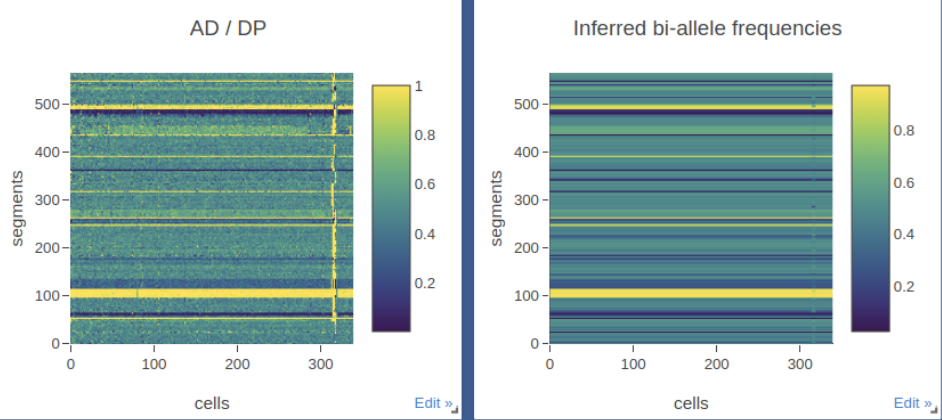
\includegraphics[keepaspectratio=true, scale=0.4]{images/unsynced_allelic_rates.png} \\
			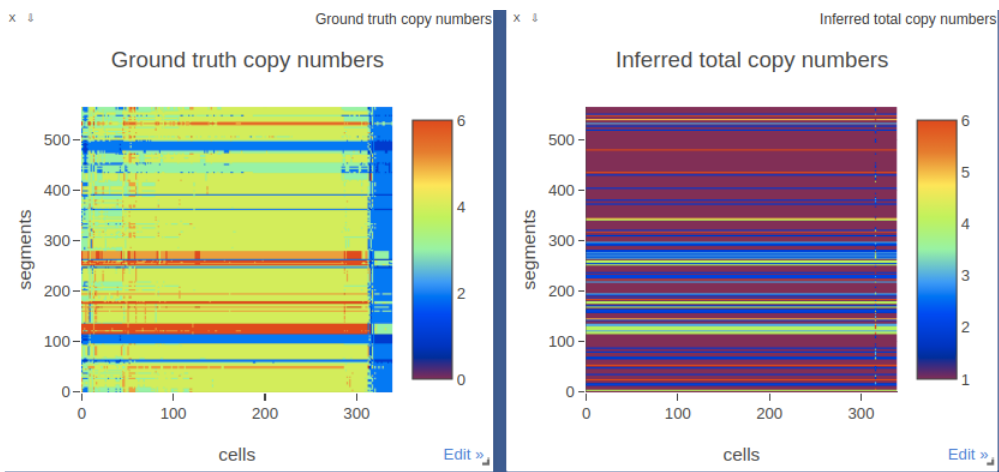
\includegraphics[keepaspectratio=true, scale=0.4]{images/unsynced_read_depths.png}
		\end{tabular}
		\caption{Несогласованность найденных VB параметров при запуске на реальных данных при использовании блок-зависимых BAF-ов (на верхних тепловых картах). Слева — ожидаемые значения, справа — предсказанные. Видно, как BAF-модуль переобучается, а RDR-модуль хоть и улавливает какие-то закономерности, но, в целом, предсказывает что-то не то (даже по модулю того, что XClone не умеет детектировать whole-genome duplication).}
	\end{figure}
	Но как только частоты аллелей в блоках стали, по сути, определяться исключительно расстановкой наиболее вероятных $Y$ и $Z$, BAF-модуль перестал переобучаться на шум в данных и изменения параметров модулей стали согласованными.
\end{itemize}

\paragraph{Численное интегрирование в оценке обоснованности RDR-модуля}
Аналитическую формулу для обоснованости RDR-модуля, увы, получить не удалось. Даже если фиксировать $\bm{m}$, неясно, как устроено отношение сумм зависимых логнормальных распределений в $\tilde f_{i, k}$. В \cite{SumOfLognormals} показано, что даже распределение числителя и знаменателя в отдельности имеет сложную структуру и не выражается через элементарные операции над стандартными распределениями. Как следствие, в коде алгоритма RDR-обоснованность приближается интегрированием по Монте-Карло. 

Это существенный недостаток XClone в текущей редакции, т.к. метод Монте-Карло в общем случае имеет корневую сходимость\footnote{Конспект лекции в MIT: \url{https://ocw.mit.edu/courses/mechanical-engineering/2-086-numerical-computation-for-mechanical-engineers-fall-2014/nutshells-guis/MIT2_086F14_Monte_Carlo.pdf}}, и для получения точности хотя бы до третьего знака приходится использовать порядка $10^{6}$ точек, и это при фиксированном $\bm{m}$. В противном случае, пришлось бы семплировать ещё больше точек, чтобы сделать поправку на размерность пространства признаков (от нескольких сотен до нескольких тысяч). 

\paragraph{Слишком большая разница масштабов отдельных слагаемых в ELBO}$ $\\
Вариационный байесовский вывод в модели XClone основан на следующем представлении ELBO:
\begin{equation}
	\mathtt{L}(q) = \int{ q(\Omega) \log p(\bm{AD}, \bm{DP}, \bm{RD}\ |\ \Omega)} \text{d} \Omega -\mathtt{KL}(q(\Omega)\ \|\ p(\Omega))
\end{equation}
При этом логарифм обоснованности распадается в сумму по BAF- и RDR-модулям:
\begin{equation} 
	\begin{split}
		&\int{ q(\Omega) \log p(\bm{AD}, \bm{DP}, \bm{RD}\ |\ \Omega)} \text{d} \Omega =\\
		&= \mathunderline{green}{\int{ q(\bm{Z}, \bm{Y}, \bm{\theta}) \log p(\bm{AD}, \bm{DP}\ |\ \bm{Z}, \bm{Y}, \bm{\theta})} \text{d} \bm Z \text{d} \bm{Y} \text{d} \bm{\theta}} + \\
		& + \mathunderline{red}{\int{ q(\bm{Z}, \bm{Y}, \bm{m}, \bm{\gamma}) \log p(\bm{RD}\ |\ \bm{Z}, \bm{Y}, \bm{m}, \bm{\gamma})} \text{d} \bm{m} \text{d} \bm{\gamma}}
	\end{split}
\end{equation}
а KL-дивергенция распадается на сумму по скрытым переменным:
\begin{equation}
	\begin{aligned}
		\mathtt{KL}(q(\Omega)\ \|\ p(\Omega)) 
		&= \mathtt{KL}(q(\bm{Z})\ \|\ p(\bm{Z})) + \mathtt{KL}(q(\bm{Y})\ \|\  p(\bm{Y})) + \\ 
		&+ \mathtt{KL}(q(\bm{m})\ \|\ p(\bm{m})) + \mathtt{KL}(q(\bm{\gamma})\ \|\ p(\bm{\gamma}))
	\end{aligned}
\end{equation}
При этом оптимальные параметры модели ищутся градиентным методом (Adam\cite{AdamOptimizer}, если быть точным). Метод не может знать о содержательном смысле параметров. Алгоритм будет в первую очередь оптимизировать те параметры, которые дают наибольший вклад в ELBO. На практике соотношение между компонентами ELBO выглядит так:
\begin{figure}[H]
	\centering
	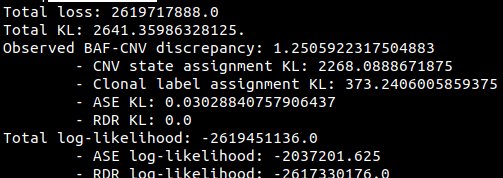
\includegraphics[keepaspectratio=true, scale=0.8]{images/loss_components_relative_scales.png}
	\caption{Величины различных слагаемых в разложении ELBO, логи модели в процессе обучения. Видно, что лог-обоснованность RDR-модуля по модулю на три порядка больше, чем аналогичная величина для BAF-модуля. Величины компонент KL-дивергенции пренебрежимо малы по сравнению с модулем лог-обоснованности модели.}
\end{figure}
Очевидный дисбаланс в величинах слагаемых приводит к тому, что алгоритм оптимизации практически не обращает внимание на KL-дивергенцию, если априорные предположения о распределениях не слишком сильные (читай, если априорные распределения не близки к вырожденным). Это приводит к тому, что апостериорные аспределения на параметрах иногда вырождаются только потому, что это почему-то позволяет сильно уменьшить лог-обоснованность одного из модулей. В силу зашумленности реальных данных, такое вырождение может происходить случайно. Это существено влияет на интерпретируемость результатов.

Кроме того, лог-обоснованность RDR-модуля доминирует над всеми остальными слагаемыми. Это не так существенно, когда $\bm{m}$ и $\bm{\gamma}$ фиксированы, а величины $\theta_{i,t}$ в BAF-модуле не являются блок-специфичными, но может быть проблемой в будущем, при добавлении новых модулей в модель (скажем, для учёта соматических мутаций или митохондриальных геномов). Тем не менее, такой дисбаланс вызван техническими факторами: элементы матрицы $\bm{RD}$ обычно заметно больше соотв. элементов матриц $\bm{AD}$ и $\bm{DP}$, но при этом <<больше>> не означает <<важнее>>.

Для борьбы с этим эффектом кажется уместным либо приводить элементы $\bm{RD}$ и $\bm{DP}$ к одному масштабу некоторым целочисленным преобразованием, либо ввести веса для компонент ELBO, хоть это и сугубо практический трюк, который нарушает логическую стройность теоретических выкладок. Также можно попробовать заменить градиентный метод Adam на квазиньютоновский L-BFGS\cite{LBFGS}. Тем не менее, планирование эксперимента, который бы показал, что один из методов лучше другого, это отдельная нетривиальная задача, к которой пока непонятно, как подступиться.

\paragraph{Концептуальная невозможность детектирования WGD}$ $\\
АЛАЛАЛАЛАЛАЛА

\paragraph{Наивный подход к определению ожидаемого числа прочтений в блоках сегментации}$ $\\
АЛАЛАЛАЛАЛАЛА

\paragraph{Отсутствие коррекции технических факторов в RDR-модуле}$ $\\
АЛАЛАЛАЛАЛАЛА

\paragraph{Необходимость вручную задавать ожидаемое число клональных линий в образце}$ $\\
АЛАЛАЛАЛАЛАЛА

\paragraph{Предположение о независимости клональных линий. Игнорирование субклональной структуры}$ $\\
АЛАЛАЛАЛАЛАЛА

\paragraph{Практические трудности вычисления плотности биномиального распределения при большой глубине покрытия}$ $\\
АЛАЛАЛАЛАЛАЛА